%%%%%%%%%%%%%%%%%%%%%%%%%%%%%%%%%%%%%%%%%%%%%%%%%%%%%%%%%%%%%%%%
%  文章模板:A4 纸,小五字
%%%%%%%%%%%%%%%%%%%%%%%%%%%%%%%%%%%%%%%%%%%%%%%%%%%%%%%%%%%%%%%%
\documentclass[a4paper, 11pt]{article}

%%%%%%%%%%%%%%%%%%%%%%%%%%%%%%%%%%%%%%%%%%%%%%%%%%%%%%%%%%%%%%%%
%  packages
%    这部分声明需要用到的包
%%%%%%%%%%%%%%%%%%%%%%%%%%%%%%%%%%%%%%%%%%%%%%%%%%%%%%%%%%%%%%%%
\usepackage[UTF8]{ctex}
\usepackage{float}
\usepackage{amsmath}
\usepackage{graphicx}
\usepackage{geometry}
\usepackage{lettrine}
\usepackage{caption}
\usepackage{subcaption}
\usepackage{setspace}
\usepackage{mathtools}
\usepackage[linesnumbered,ruled,vlined]{algorithm2e}
\usepackage{algorithmic}
\usepackage[backend=biber,style=authoryear]{biblatex}
\usepackage{listings}
\usepackage{color}
\usepackage{hyperref}
\addbibresource{citation.bib}

%%%%%%%%%%%%%%%%%%%%%%%%%%%%%%%%%%%%%%%%%%%%%%%%%%%%%%%%%%%%%%%%
%  lengths
%    下面的命令重定义页面布局
%%%%%%%%%%%%%%%%%%%%%%%%%%%%%%%%%%%%%%%%%%%%%%%%%%%%%%%%%%%%%%%%
\geometry{scale=0.8}
\linespread{1.5}


%%%%%%%%%%%%%%%%%%%%%%%%%%%%%%%%%%%%%%%%%%%%%%%%%%%%%%%%%%%%%%%%
%  杂项
%%%%%%%%%%%%%%%%%%%%%%%%%%%%%%%%%%%%%%%%%%%%%%%%%%%%%%%%%%%%%%%%

\definecolor{codegreen}{rgb}{0,0.6,0}
\definecolor{codegray}{rgb}{0.5,0.5,0.5}
\definecolor{codepurple}{rgb}{0.58,0,0.82}
\definecolor{backcolour}{rgb}{1,1,1}

\SetKwInput{KwInput}{Input}                % Set the Input
\SetKwInput{KwOutput}{Output}  
\SetKwInput{KwDeclare}{Declare} 

\DeclarePairedDelimiter{\ceil}{\lceil}{\rceil}
\DeclarePairedDelimiter{\floor}{\lfloor}{\rfloor}
\newcommand\mycommfont[1]{\footnotesize\ttfamily\textcolor{blue}{#1}}
\SetCommentSty{mycommfont}

%%%%%%%%%%%%%%%%%%%%%%%%%%%%%%%%%%%%%%%%%%%%%%%%%%%%%%%%%%%%%%%%
%  代码高亮
%%%%%%%%%%%%%%%%%%%%%%%%%%%%%%%%%%%%%%%%%%%%%%%%%%%%%%%%%%%%%%%%
% \usepackage[cache=false]{minted}
% \newminted[CPP]{c++}{mathescape, linenos, numbersep=5pt, gobble=0, tabsize=4, fontsize=\small, frame=lines,framesep=2mm}
% \newminted[PY]{python}{mathescape, linenos, numbersep=5pt, gobble=0, tabsize=4, fontsize=\small, frame=lines,framesep=2mm}
% \newminted[SQL]{sql}{mathescape, linenos, numbersep=5pt, gobble=0, tabsize=4, fontsize=\small, frame=lines,framesep=2mm}

\hypersetup{
	colorlinks=true,
	linkcolor=black
}


%%%%%%%%%%%%%%%%%%%%%%%%%%%%%%%%%%%%%%%%%%%%%%%%%%%%%%%%%%%%%%%%
%  文章主体
%%%%%%%%%%%%%%%%%%%%%%%%%%%%%%%%%%%%%%%%%%%%%%%%%%%%%%%%%%%%%%%%
\title{	
\normalfont \normalsize
\textsc{School of Data and Computer Science, Sun Yat-sen University} \\ [25pt] %textsc small capital letters
\rule{\textwidth}{0.5pt} \\[0.4cm] % Thin top horizontal rule
\huge  基于CUDA加速的改进Mean Shift图像分割算法\\ % The assignment title
\rule{\textwidth}{2pt} \\[0.5cm] % Thick bottom horizontal rule
\author{ \textbf{组长: }\ 16337180麦显忠\\ 16313018李沐晗,\ 16337242韦博耀,\ 16337259谢江钊, \ 16337179麦金杰}
\date{\normalsize\today}
}

\begin{document}
\maketitle


\tableofcontents
\newpage


\section{Introduction}

\subsection{Mean Shift算法概述}
Mean Shift算法用于图像分割最早是由~\autocite{comaniciu2002mean}提出的. 算法的主要步骤可以分为三步:
\begin{enumerate}
    \item Mean Shift滤波
    \item 将像素点聚类为区域
    \item 进行标签分配
\end{enumerate}

下文介绍这篇PAMI论文提出的使用Mean Shift进行图像分割的原理及具体实现.

\subsubsection{Mean Shift滤波}
Mean Shift滤波即mode搜索过程. Mean Shift算法将图像分割视为一个聚类问题. 要进行聚类, 需要先找到聚类中心, 也就是
所称的mode, 再由此出发进行聚类的过程. 在原文中, 作者先将原图映射到特征空间, 再从这个映射得到的特征空间中搜索mode点.

\begin{figure}[!htb]
    \label{fig:figure1}
\centering
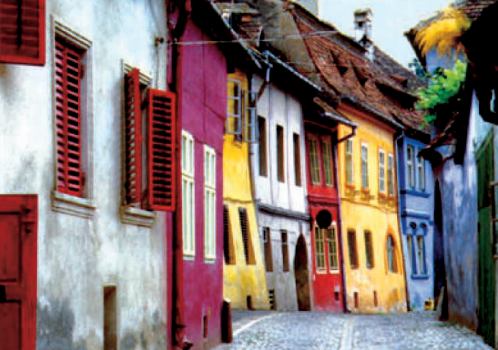
\includegraphics[width=0.5\textwidth]{images/origin.png}
\caption{原图}
\end{figure}

我们参照了原文作者的方法,将LUV颜色空间作为待搜索的特征空间. LUV空间中像素点的分布如图\ref{fig:luv lu}所示, 原始输入图像位于RGB空间,使用LUV空间的优点为,LUV为均匀的色度空间,色差可用欧式距离计算. 

以下我们将描述mode点搜索过程, 为方便讨论, 我们仅考虑三维的LUV特征空间的L和U维,如图\ref{fig:luv lu},
图\ref{fig:mode}为图\ref{fig:lu}的密度表示,若将邻域内点的密度作为搜索聚类中心
mode的标准, 那么图\ref{fig:mode}中的红色点即我们需要搜索的聚类中心.

\begin{figure}
    \centering
    \begin{subfigure}[b]{0.4\textwidth}
        \centering
        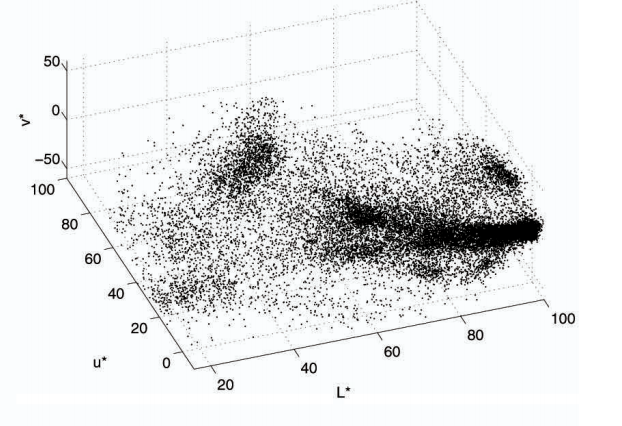
\includegraphics[width=\textwidth]{images/luv.png}
        \caption{LUV}
        \label{fig:luv}
    \end{subfigure}
    \hfill
    \begin{subfigure}[b]{0.4\textwidth}
        \centering
        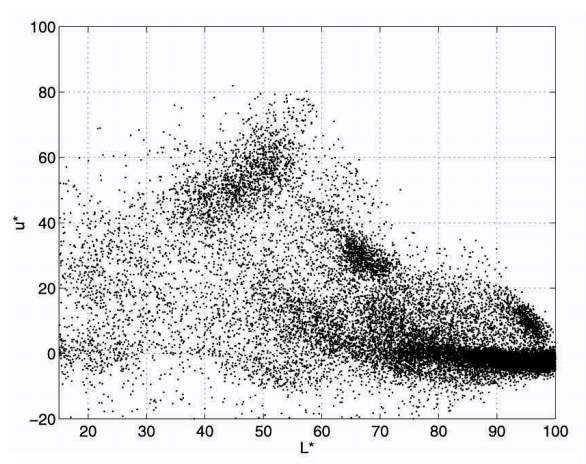
\includegraphics[width=\textwidth]{images/lu.png}
        \caption{LU}
        \label{fig:lu}
    \end{subfigure}
\caption{LUV and LU}
\label{fig:luv lu}
\end{figure}

\begin{figure}[!htb]    
    \centering
    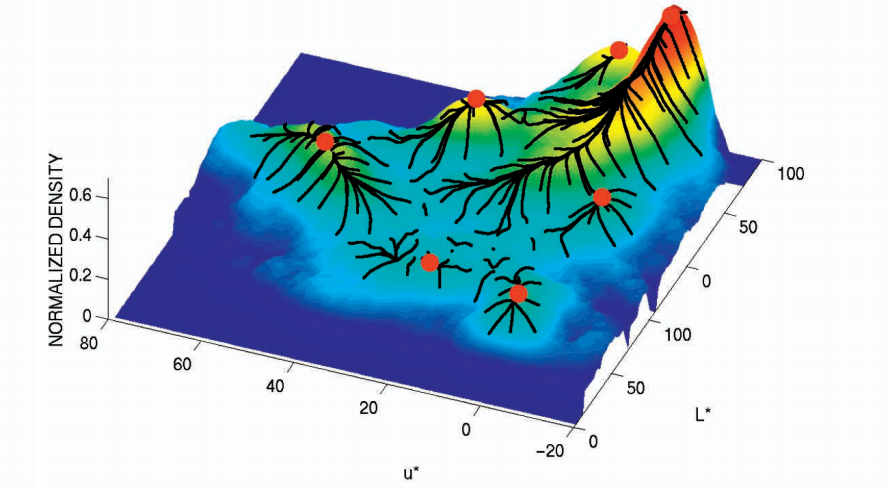
\includegraphics[width=0.5\textwidth]{images/mode.png}
    \caption{Mode}
    \label{fig:mode}
\end{figure}



在原来Mean shift算法的实现中, 作者采用了基于核密度估计的策略来寻找mode点. 首先, 给出以下核函数公式:
\begin{equation} \label{eq:1}
    \hat{f}(x)=\frac{1}{nh^d}K(\frac{x-x_i}{h})
\end{equation}

其中x代表输入数据, n是数据点数, h是带宽, d是数据的维度. 基于公式\ref{eq:1},作者提出了新的核密度估计方法. 首先有:
\begin{equation}\label{eq:2}
    \hat{f}(x)=\frac{c_{k,d}}{nh^d}k(||\frac{x-x_i}{h}||^2)
\end{equation}

\begin{equation}\label{eq:3}
    \hat{\bigtriangledown }f_{h,K}(x)=\frac{2c_{k,d}}{nh^{d+2}}\sum^n_{i=1}(x-x_i)k'(||\frac{x-x_i}{h}||)
\end{equation}

\begin{equation}\label{eq:4}
    g(x)=-k'(x)
\end{equation}
    
\begin{equation}\label{eq:5}
    G(x)=c_{g,d}g(||x||^2)
\end{equation}

 这里我们用\ref{eq:5}中的G(x)作为新的核函数. 而根据上面的符号我们可以将重写~\ref{eq:2}的导数为
\begin{equation}\label{eq:6}
    \begin{split}
        \hat{\bigtriangledown }f_{h,K}(x)\\
        &=\frac{2c_{k,d}}{nh^{d+2}}\sum^n_{i=1}(x_i-x)g(||\frac{x-x_i}{h}||^2)\\
        &=\frac{2c_{k,d}}{nh^{d+2}}[\sum^n_{i=1}g(||\frac{x-x_i}{h}||^2)][\frac{\sum_{i=1}^nx_ig(||\frac{x-x_i}{h})||^2}{g(||\frac{x-x_i}{h})||^2}-x]
    \end{split}
\end{equation}

因此, 算法中的第二项就是我们算法中所称的Mean shift $m_{h,G}(x)$, 由上面的推导可以得到:

\begin{equation}\label{eq:7}
    \begin{split}
    m_{h,G}(x)&=\frac{\sum_{i=1}^nx_ig(||\frac{x-x_i}{h})||^2}{g(||\frac{x-x_i}{h})||^2}-x\\
    &=\frac{1}{2}h^2c\frac{\hat{\bigtriangledown }f_{h,K}(x)}{\hat{f}_{h,G}(x)}
    \end{split}
\end{equation}

从式~\ref{eq:7}我们就可以看到, Mean shift与数据密度的梯度方向相同, 这就证明了从任意点开始, 只要朝mean shift的方向移动, 就会慢慢的走向密度估计最大的地方, 而这也正是我们需要找的聚类中心, 也就是之前提到的mode点. 一个更加形式化的说明见图\ref{fig:search}, 可以看到, 不断朝着mean shift的方向进行
移动, 最终到达了密度最大处.

\begin{figure}[H]
    \centering
    \begin{subfigure}[b]{0.4\textwidth}
        \centering
        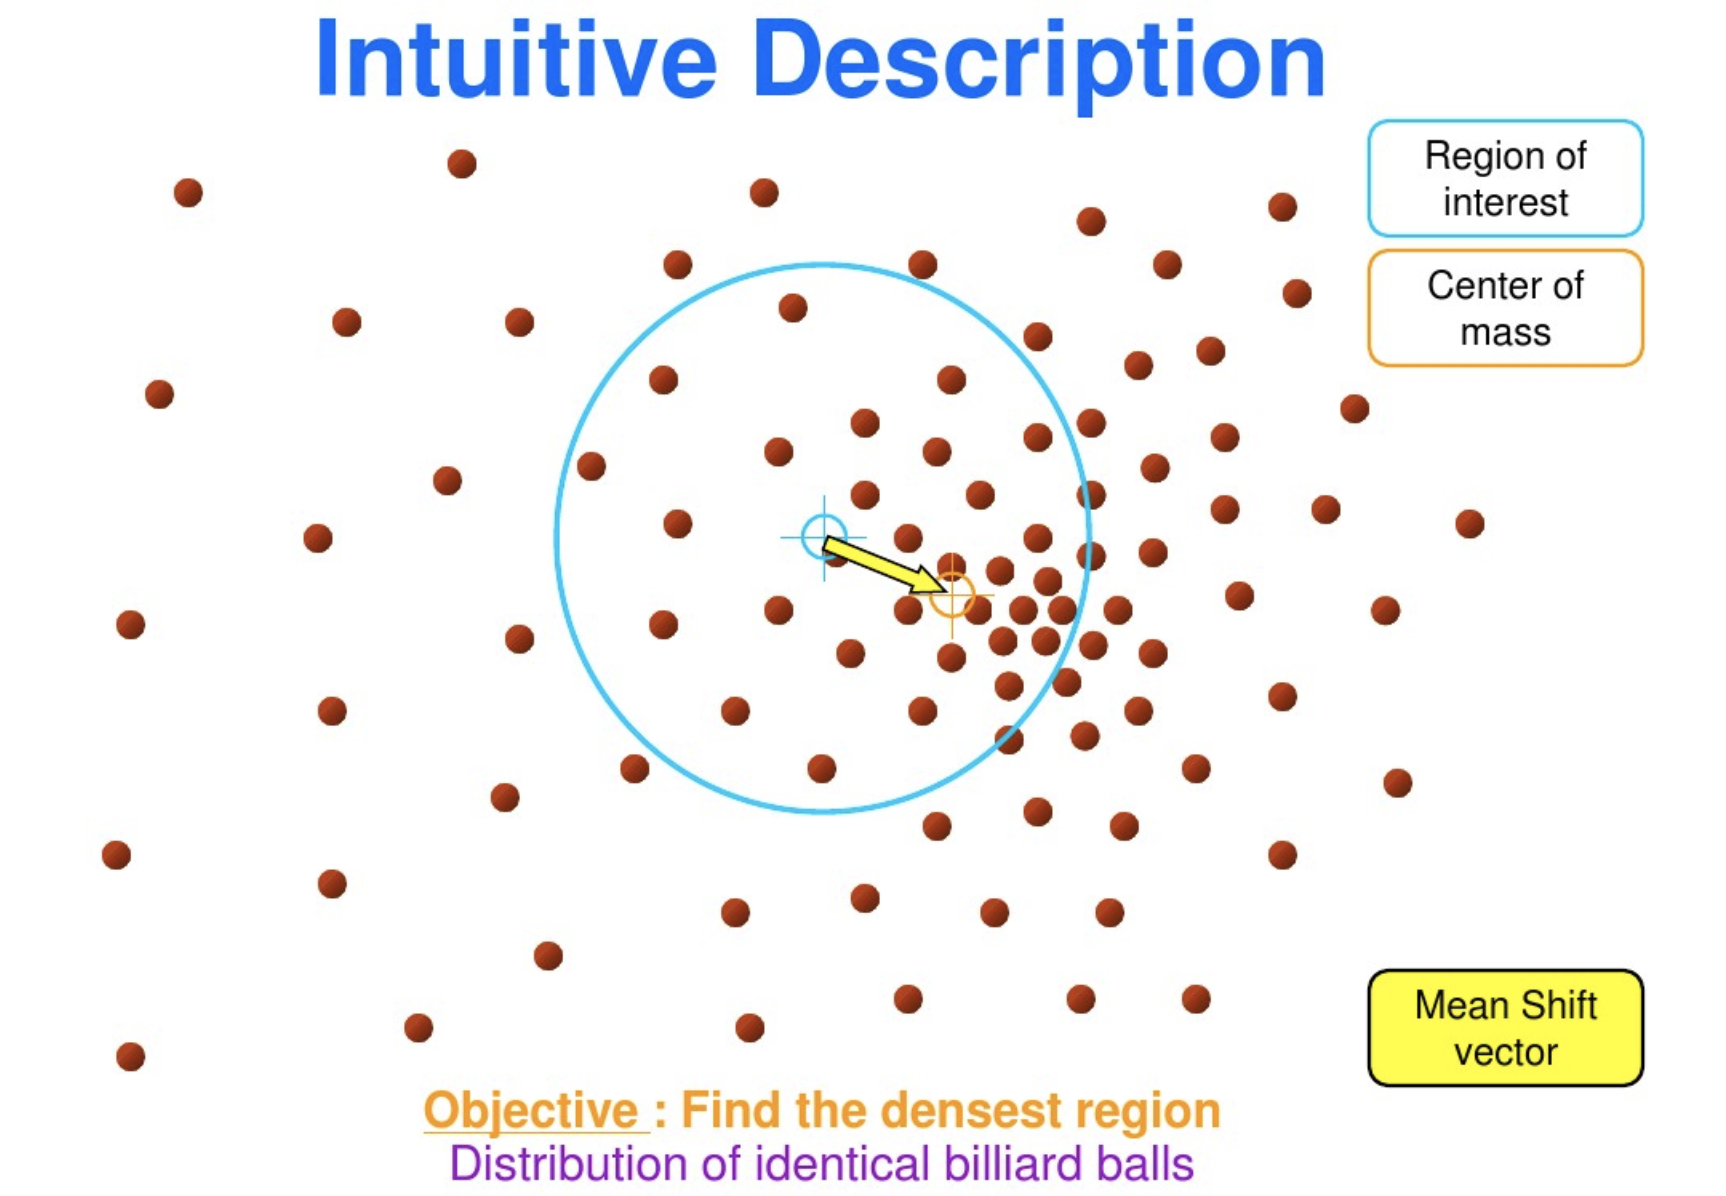
\includegraphics[width=\textwidth]{images/mean1.png}
        
    \end{subfigure}
    \hfill
    \begin{subfigure}[b]{0.4\textwidth}
        \centering
        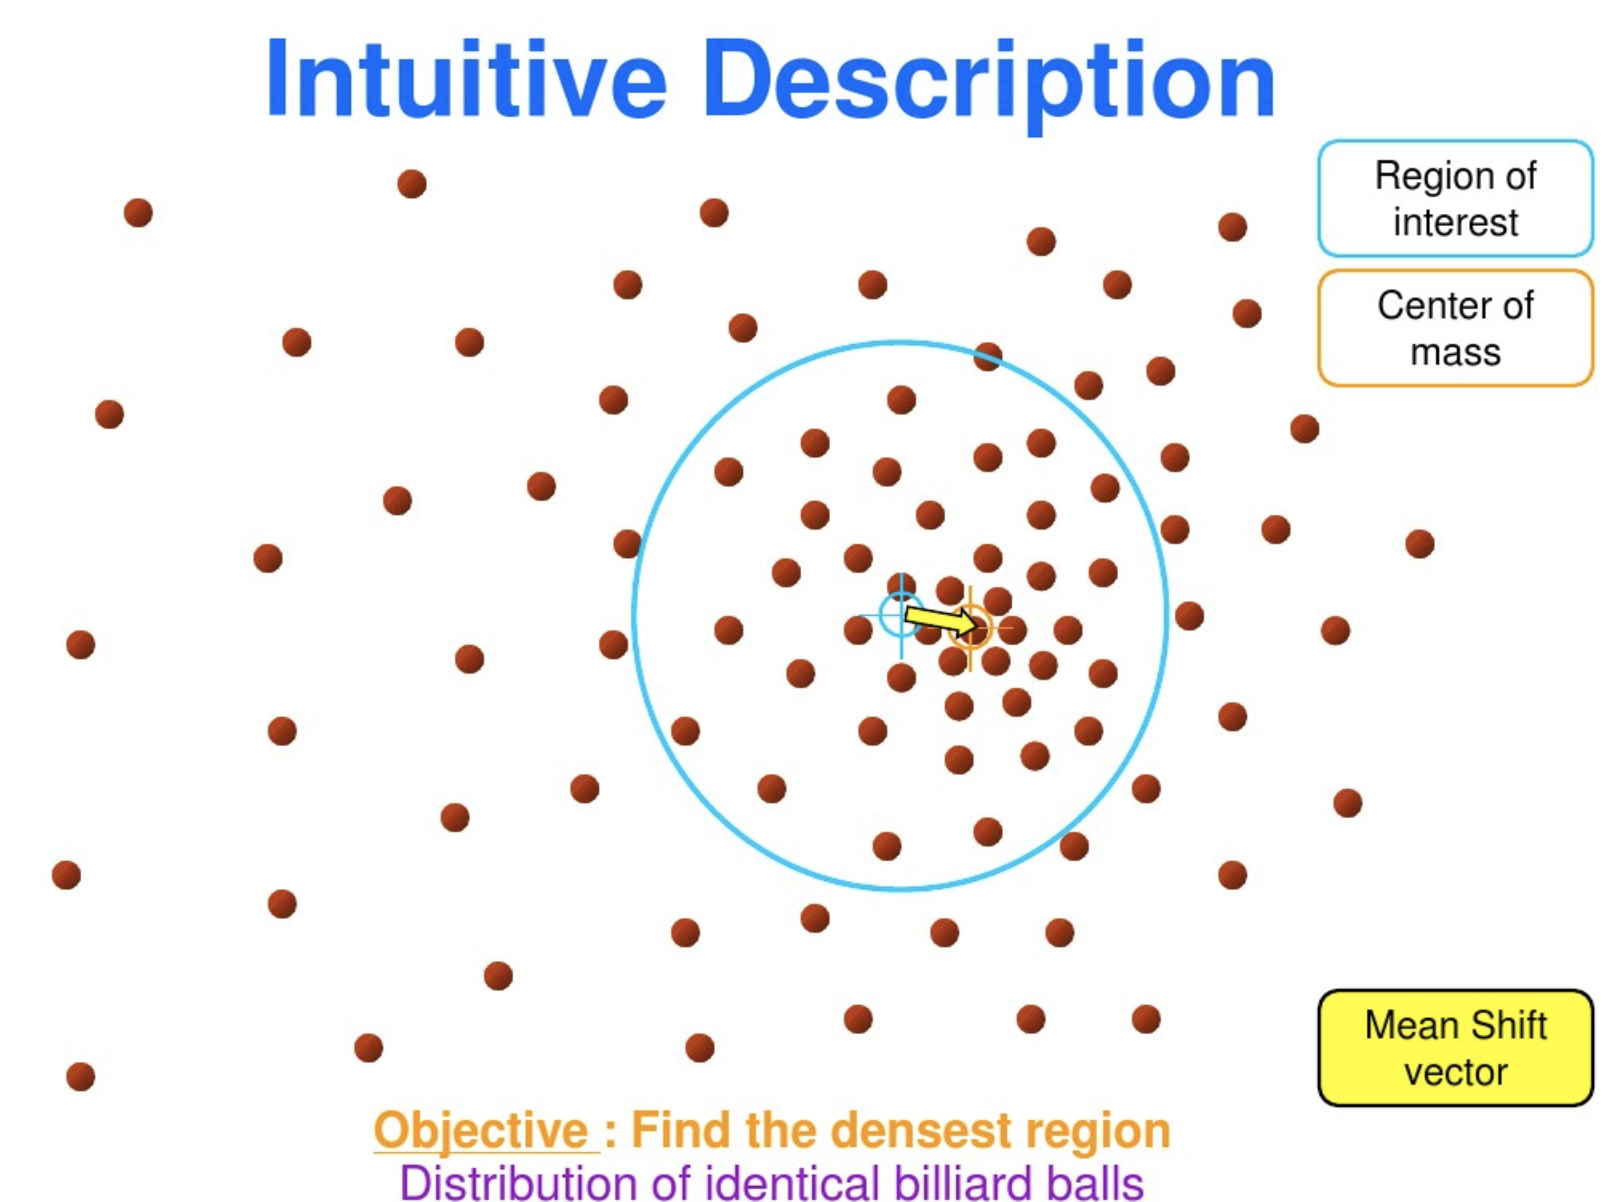
\includegraphics[width=\textwidth]{images/mean2.png}
    
    \end{subfigure}
\caption{搜索}
\label{fig:search}
\end{figure}

\subsubsection{聚类和分割}

经过上面的步骤后, 对于输入数据中的每个点(如图片中的像素点), 我们都能找到它的mode点, 即聚类中心. 接下来我们就可以开始围绕着聚类中心进行聚类.
原文中的具体方法是根据空间距离和颜色距离这两个度量指标, 采取类似于种子生成的策略一步步的将mode点附近的像素加入到各个mode当中, 最后对
这些以mode为中心的, 零碎的小区域进行平滑和合并, 就得到了最终的分割图像. 比较直观的可视过程可以参见下图\ref{fig:process}.

\begin{figure}[!htb]    
    \centering
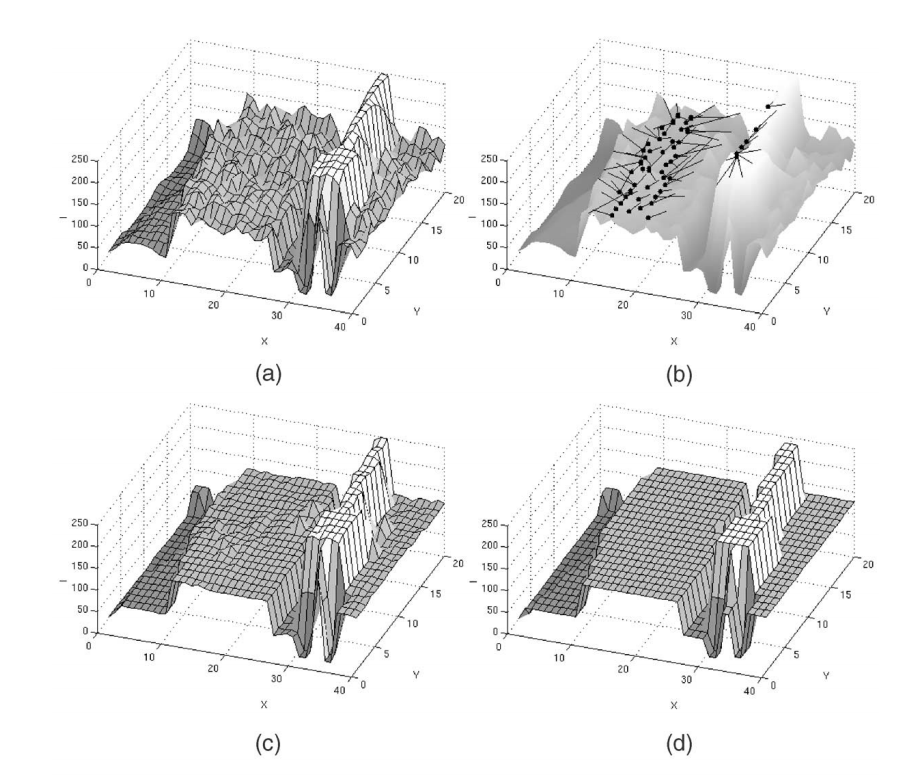
\includegraphics[width=0.7\textwidth]{images/pro.png}
\caption{流程}
\label{fig:process}
\end{figure}

其中a图即是原图像经映射后得到的特征空间, b图表示了从图像的各个点出发, 同时寻找对应的mode点的过程. c图表示了根据距离相似性和色彩空间相似性
得到的聚类结果, d图即是经过了平滑, 极小区域擦除后的最终分割图像. 一个完整的例子可以参见下图\ref{fig:example}.

\begin{figure}[!htb]  
    \centering
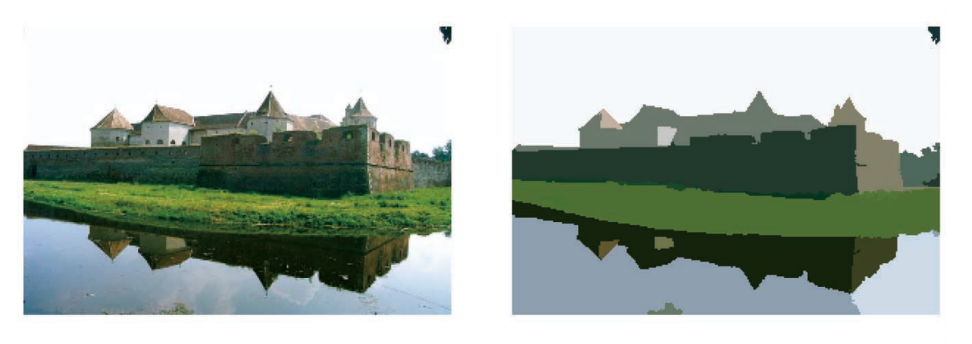
\includegraphics[width=0.7\textwidth]{images/example.png}
\caption{例子}
\label{fig:example}
\end{figure}

\subsection{课程实验}
因此, 我们组决定参照此篇论文提出的基于Mean shift的图像分割算法, 进行一定的复现和改进. 我们计划实现的算法大体框架如下:

\subsubsection{Mean shift滤波 } 

\begin{algorithm}[H]
    \DontPrintSemicolon
	\setstretch{1.15}
    \KwInput{图片I}
    \KwOutput{Meanshift分割后的图片I'}
    \For{I中的每个像素点(x,y)}
    {
        \While{没有达到迭代次数上限}
        {
            像素点(x,y)当前的LUV值为$I_{x,y}$\;
            设置color\_sum = [0,0,0], index\_sum = [0, 0], summed\_pixels = 0\;
            \For{对以带宽dh为半径的圆或正方形邻域内的像素点(x',y')}
            {
                计算$\Delta LUV=||I_{x,y}-I_(x',y')|$\;
                \If{$\Delta LUV>color\_max\_diff\_range$}
                {
                    $color\_sum += I_{x',y'}$\;
                    $index\_sum += (x',y')$\;
                    $summed\_pixels++$\;
                }
                $cs\_avg=\frac{color\_sum}{summed\_pixels}$\;
                $is\_avg=\frac{index\_sum}{summed\_pixels}$\;
                $shift = |cs\_avg|^2 + |is\_avg|^2$ \;
                更新$I'_{x,y}=cs\_avg$\;
                \If{$shift<shift\_range$}
                {
                    \textbf{break}\;
                }
            }
        }
    }
    \Return{输出图像I'}
\caption{Meanshift算法}
\label{code1}
\end{algorithm}

和原算法一致, 这一步同样是为了找到聚类中心. 在本次实验中我们采取了稍有不同的实现.
首先, 我们只采用LUV颜色空间作为特征, 据此先给出算法的伪代码\ref{code1}.

可以看到, 在我们的实现伪代码\ref{code1}中, 每个点的像素值不断地朝区域平均值的方向移动, 也即mean shift.
待到算法终止时, 每个像素点的像素值都mean shift到了某一簇像素.

\subsubsection{聚类 (Flooding)} 

\begin{algorithm}[H]
    \DontPrintSemicolon
    \setstretch{1.15}
    \KwInput{经过Mean shift后的图片I}
    \KwOutput{图片I上每个像素点对应的label}
    \For{I中的每个像素点(x,y)}
    {
        分配一个唯一的$label_{x,y}=y*width+x$\;
        \While{没有达到迭代次数上限}
        {
            \For{对以带宽dh为半径的圆或正方形邻域内的像素点(x',y')}
            {
                \If{$\Delta LUV<color\_max\_diff\_range$}
                {
                    更新$label_{x',y'}=label_{x,y}$\;
                }
            }
        }
    }
    \Return{图像I对应的label}
\caption{Flooding 洪泛搜索}
\label{code2}
\end{algorithm}

完成初步的滤波后, 我们还需要对每一个像素都分配一个特定的标签, 以此完成图像分割
的任务要求. 而由于Mean shift方法本质上是无监督的算法, 因此我们只能给每个像素分配没有实际意义的标签. 实践中,我们使用坐标给予每个像素点一个独特的初始标签,这一步骤的
具体过程如伪代码\ref{code2}所示.

在以上步骤中, 不难发现, 如果对上述过程进行并行化, 可能会有多个像素点抢一个像素点的情况(赋给自己的label), 
这会由线程间的竞争决定最后谁赋值成功. 也就是说, 对于相同的输入, 标签分配算法并不能保证得到完全相同的输出.
但需要说明的是, 这里线程的竞争导致的标签不一致, 可以在后续步骤的区块合并中得到解决.

但在实际实验中, 我们发现如果对每个像素都进行并行化, 会造成比较密集的冲突和重复赋值, 降低并行化的
效率. 为了解决这一情况, 我们在实际中进行了优化. 在某一部分像素点钟, 只让一个像素点线程进行洪泛搜索. 这些
搜索部分的划分可以由行和列确定, 例如每个$n*n$的子图像只让一个像素点进行标签洪泛. 在循环中采取类似
卷积移动滑动窗口的方式, 对下一个部分进行标签分配.


\subsubsection{区域合并} 

\begin{algorithm}[H]
    \DontPrintSemicolon
	\setstretch{1.15}
    \KwInput{经过Mean shift后的图片I}
    \KwInput{经过Flooding的label}
    \KwOutput{最终经过聚合的label}
    创建栈stack\;
    \For{I中的每个像素点(x,y)}
    {
        分配一个唯一的$label_{x,y}=y*width+x$\;
        stack.push($I_{x,y}, label_{x,y}$)\;
    }
    \While{!stack.empty()}
    {
        从stack中取出像素值$x_i, y_i$和标签$x_l, y_l$\;
        计算$\Delta LUV=||x_i-y_i)||$\;
        \If{$\Delta LUV<color\_max\_diff\_range$}
        {
            UnionFind($x_l, y_l$)\;
        }
    }
    \Return{图像I对应的label}
\caption{区域合并算法}
\label{code3}
\end{algorithm}

最后一步, 根据上一步得到的聚类结果, 我们再进行最后一步后处理得到最后的分割. 
对于过小的区块和相似的区块, 我们将它和邻近的进行合并, 并对分割图像进行一定的平滑和滤波处理. 即得到了分割结果.

在这一部分中, 我们采用了并查集算法(UnionFind),并查集算法在\autocite{Galler:1964:IEA:364099.364331}中可以找到详细的描述,区域合并算法的过程如伪代码\ref{code3}所示。

我们采用了pthread的多线程并行和CUDA并行对上面的算法进行优化, 因为CUDA并行结构和CPU多线程并行的细节之处十分不同,因此此处只介绍主要的并行化思想,在实现部分将具体介绍使用的算法:
\begin{enumerate}
    \item 将待聚合标签数据进行分块,进行本地聚合处理
    \item 对所有标签数据进行全局聚合处理
    \item 统计区域数量,并对标签进行重新映射
\end{enumerate}

\clearpage
\section{Implementation}
本节中,我们将对算法各个部分的具体实现进行详细描述。

\subsection{Mean Shift滤波的并行化}

\subsubsection{并行优化思路}
\begin{enumerate}
    \item Mean shift算法在迭代过程中会用到固定范围内的二维矩阵元素,这种读取方式如果采用一维读入二维转换的 方法读取,性能不会特别好,而相比之下,纹理内存的存在可以极大地提高这种二维相邻的读取速度,充分利 用缓存。
    \item 同一个block内的线程下的元素,它们在执行算法循环的同时,使用到的数据大多是重复的,也就是说一个 block内不需要把所有数据全部读取上来,可以使用共享内存进一步进行加速。
    \item 对于循环内部,因为没有存在读写数据依赖,可以采用循环展开进行加速。
    \item 对于浮点数值,可以添加f作为后缀说明,减少强制转换的开销。
\end{enumerate}

\subsubsection{算法流程}

\begin{enumerate}
    \item CImg读入图像数据,以RRRGGGBBB..的形式保存为float*数组。使用cudaMallocPitch函数和cudaMemcpy2D()函数在device开辟二维空间,读入该数组。
    \item 通过上述内存空间创建纹理对象。
    \item Block内创建二维共享内存,第一个维度为通道,第二个维度为BLock内需要访问的每个通道的数据大小,大小 为BLock的长宽分别加上dis\_range的乘积。
    \item 共享内存写好后,执行算法的主要部分,迭代漂移到区域内的某个颜色值的相近点,最后将结果输出。
\end{enumerate}

下面给出的算法的详细伪代码.

\begin{algorithm}[H]
	\setstretch{1.15}
	\DontPrintSemicolon
    \KwInput{Cimg读入的图片in\_tex,最大颜色区别 color\_range,图片尺寸 height,width,}
    \KwOutput{经过滤波的output}
    \KwDeclare{pixels[][] 位于共享内存}
    $col,row$ $\leftarrow$ 2D global $thread\_id$ \;
    \If{ col >= width or row >= height then}{
        \Return{}
    }
    
    $patch\_height,patch\_width \leftarrow blk\_w+2*dis\_range,blk\_h+2*disrange$ \;
    共享内存读入;  \tcp{read data}
    syncthreads()\;
    $cur\_row,cur\_col \leftarrow threadIdx.y+dis\_range,threadIdx.x+dis\_range$ \; 
    $L,U,V \leftarrow pixels[][cur\_row*patch\_width+cur\_col]$ \;
    $shift \leftarrow 5$ \;
    $col\_from,col\_to \leftarrow threadIdx.x,threadIdx.x+2*dis\_range+1$ \;
    $row\_from,row\_to \leftarrow threadIdx.y,threadIdx.y+2*dis\_range+1$ \;
    
    \For{ iter 0 to max\_iter and shift<3 }{
        $old\_row,old\_col \leftarrow cur\_row,cur\_col$ \tcp{loop to update L,U,V}
        $old\_L,old\_U,old\_V \leftarrow L,U,V$ \;
        $avg\_row,avg\_col,avg\_L,avg\_U,avg\_V,num \leftarrow 0$ \;
        \For{r row\_from to row\_to}{
            \For{ c col\_from to col\_to}{
                L2,U2,V2=pixel[][r*patch\_width+c] \tcp{scan area data}
                $d\_L,d\_U,d\_V \leftarrow L2,V2,U2-L,U,V$ \;
                \If{ $(d\_L,d\_U,d\_V)^2 <= color\_range$}{
                    $avg\_row,avg\_col+=r,c$ \;
                    $avg\_L,avg\_U,avg\_V+=L2,U2,V2$ \;
                    $num++$ \;
                }
            }
        }
        $num\_ \leftarrow 1/num$ \tcp{calculate avg}
        $L,U,V \leftarrow avg\_* num$ \;
        $cur\_row,cur\_col \leftarrow round(avg\_row*num\_),round(avg\_col*num\_)$ \;
        $d\_row,d\_col \leftarrow cur\_row,cur\_col-old\_row,old\_col$ \;
        $d\_L,d\_U,d\_ \leftarrow L,U,V - old\_L,old\_U,old\_V$ \;
        $shift \leftarrow (d\_row,d\_col,d\_L,d\_U,d\_V)^2$ \;
        
    }
    output[row,col] $\leftarrow$ L,U,V
\caption{Mean Shift并行算法}
\label{code:cuda_ms}
\end{algorithm}


其中关于Mean shift算法的主要部分,流程如下:

\begin{enumerate}
    \item 对于每一个数据点,获取自己的LUV颜色值,命名为L,U,V,获取自己的row,col坐标值
    \item 数据点需要迭代的区域范围为 $[threadIdx.x][threadIdx.y]$ 到 $[threadIdx.x+2*dis_range+1] [threadIdx.y+2*dis_range+1]$ 。
    \item 遍历区域范围内的每一个点,对每一个数据点,获取它的LUV,
    命名为L2,U2,V2,计算与L,U,V的三维上
    的距离是否小于color\_range,如果成立
    则向avg\_row,avg\_col,avg\_L,avg\_U,avg\_V中加入该点的数据,
    另外记录加入的点的数目num++。
    \item 迭代结束后,avg\_*变量中的值实际上为符合条件的点的数值的和,
    因此使用num\_变量作为num变量的倒数减 少除法计算,
    随后利用avg\_*与num\_的乘积计算出平均的LUV和坐标值,并赋值到L,U,V变量和坐标值中 去,
    并根据原L,U,V和新L,U,V的二维距离+原row,col和新row,col的距离计算shift
    \item 以上3-5作为一个循环,反复计算,也就是不断进行漂移,计算新的LUV和row,col值。当shift<=3或 iters>=max\_iter时跳出循环。
    \item 最终获取到漂移结束的LUV值,将该值赋给线程处理的像素点,输出到结果,也就完成了算法的主要内容。
\end{enumerate}

\subsubsection{共享内存的读入}
对于共享内存的读入这一方面,采用了更好的方法:


\begin{figure}[H]    
    \centering
    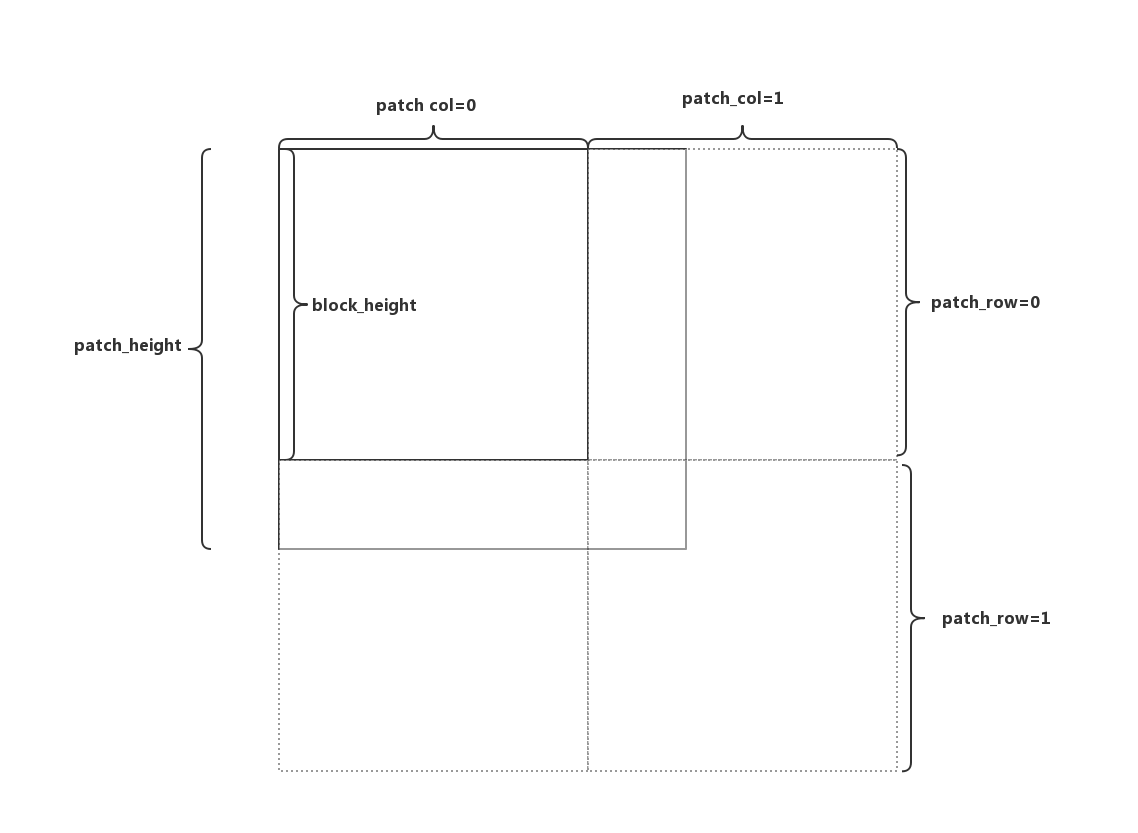
\includegraphics[width=0.5\textwidth]{images/patch.png}
\end{figure}

共享内存需要读入的数据,也就是block对应在图像中的位置延伸dis\_range的大矩形的数据,对于这样的数据,我们
让block中的所有线程每次读取若干个元素,元素数量跟dis\_range的范围有关,即可完成数据的读取.

由于这个部分较为复杂,以下结合具体代码进行分析.

blk\_x\_idx,blk\_y\_idx为线程所在block在全局中对应的位置,也是在图像中对应的位置.

\begin{CPP}
    int blk_x_idx = blockIdx.x * blockDim.x;
    int blk_y_idx = blockIdx.y * blockDim.y;
    int col = blk_x_idx + threadIdx.x;
    int row = blk_y_idx + threadIdx.y;
\end{CPP}

start\_col,start\_row为blk\_x\_idx,blk\_y\_idx分别减去dis\_range的数值,
表示对于每个数据点,读取从自己的左上方开始,也正好是block整体需要的数据的边界。
\begin{CPP}
    int start_col = blk_x_idx - dis_range;
    int start_row = blk_y_idx - dis_range;
    const int patch_width = blk_w + 2 * dis_range;
    const int patch_height = blk_h + 2 * dis_range;
\end{CPP}

 patch\_cols,patch\_rows是修正过后的patch\_width/blk\_w和patch\_height/blk\_h的值,
 用于计算出来共享内存 尺寸和block尺寸的比值,
 因为block的线程数量有限,
 一个线程读取一个数据则只能覆盖好block范围内的点, 
 这个做法的思想是把共享内存划分成若干个区域,通过这个值可以进行迭代,
 每个点去覆盖剩下的区域,确保 所有区域被覆盖完全,也就把整个共享内存写入完全。

\begin{CPP}
    const int patch_cols = (patch_width + (blk_w - 1)) / blk_w;
    const int patch_rows = (patch_height + (blk_h - 1)) / blk_h;
\end{CPP}

随后开始循环,设置循环变量i,j,范围对应为0到patch\_rows和patch\_cols,
然后对于每一个区域,计算 p\_col,p\_row,
对应将要读入的数据在共享内存中的坐标值,
然后可以计算出共享内存的p\_offset。
另一方面, read\_col,
read\_row对应从start\_col,start\_row加上p\_col,p\_row,对应的是在纹理内存中的位置。

\begin{CPP}
    for(int i=0; i<patch_rows; i++) {
        for(int j=0; j<patch_cols; j++) {
            const int p_col = j * blk_w + threadIdx.x;
            const int p_row = i * blk_h + threadIdx.y;
            const int read_col = start_col + p_col;
            const int read_row = start_row + p_row;
            if (p_col < patch_width && p_row < patch_height) {
                const int p_offset = p_row * patch_width + p_col;
                pixels[0][p_offset] = tex2D<float>(in_tex, read_col, read_row) * 100 / 255;
                pixels[1][p_offset] = tex2D<float>(in_tex, read_col, read_row + height) - 128;
                pixels[2][p_offset] = tex2D<float>(in_tex, read_col, read_row + height2) - 128;
            }
        }
    }
\end{CPP}

\subsubsection{优化总结}

算法在将像素点分配到线程实现并行加速的基础上,进行了以下若干优化:

\begin{enumerate}
    \item 读取图像数据时,因为算法读取的数据点在二维上相近,使用纹理内存加速后续读取。
    \item 每个Block内部的线程处理的像素点所需要的数据都在一定的范围内,使用共享内存来提高读取速度,
    另外对于 共享内存的写入采用新的方法减少重复读取。
    \item 算法内部的循环采用循环展开进行加速。
\end{enumerate}

\subsubsection{加速结果}
在CPU为XEON E5 E5-2620 v4, GPU为TITAN X (Pascal)平台上, 块大小配置为\{32,32,1\}运行结果为:

\begin{table}[H]
	\centering
	\begin{tabular}{ccccc}
		\hline
		图像大小   & filter range & CPU单线程版本(ms) & GPU版本(ms) & 加速比 \\ \hline
		640x480   & 2            & 315.9           & 0.469       & 673.5 \\ \hline
		640x480   & 4            & 942.1           & 0.879       & 1071.7\\ \hline
		640x480   & 8            & 3539.3          & 5.237       & 675.8 \\ \hline
		640x480   & 16           & 13250.5         & 21.614      & 613.0 \\ \hline
		1920x1080 & 2            & 799.9           & 1.058       & 756.0 \\ \hline
		1920x1080 & 4            & 2332.4          & 4.873       & 478.6 \\ \hline
		1920x1080 & 8            & 8018.2          & 15.144      & 529.4 \\ \hline
		1920x1080 & 16           & 30611.5         & 61.714      & 496.0 \\ \hline

	\end{tabular}
	\caption{Meanshift运行时间表}
	\label{tb:meanshift}
\end{table}

产生的效果如图\ref{fig:cuda_ms_1}所示:

\begin{figure}[H]
	\centering
	\begin{subfigure}[b]{0.4\textwidth}
		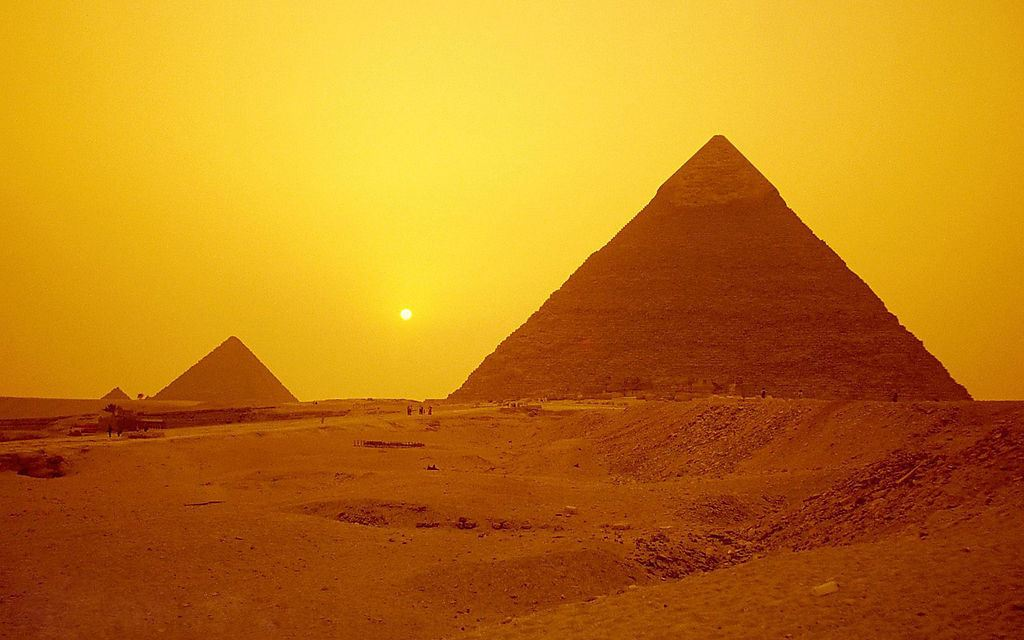
\includegraphics[width=\textwidth]{images/cuda_ms/1_org}
		\caption{original image}
	\end{subfigure}
	\hspace{5mm} 
	\begin{subfigure}[b]{0.4\textwidth}
		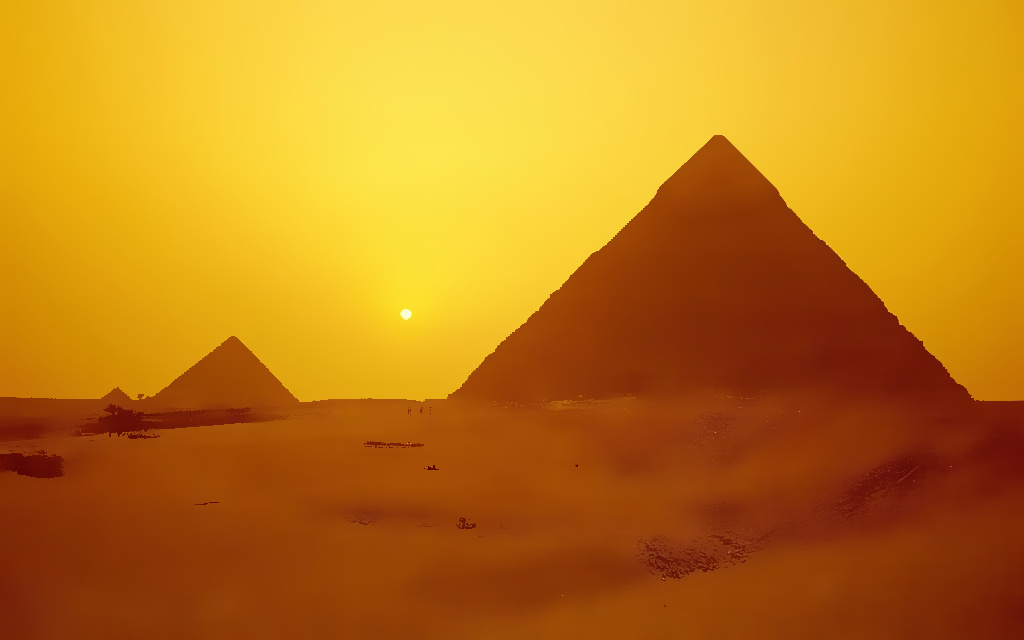
\includegraphics[width=\textwidth]{images/cuda_ms/1_res}
		\caption{filtered result}
	\end{subfigure}
	\caption{meanshift result(dis\_range=16, color\_range=500)}
	\label{fig:cuda_ms_1}
\end{figure}

\subsection{聚类flooding的并行化}
\subsubsection{并行优化思路}
从原始算法中我们得知洪泛搜索需要以像素点为中心,
和固定半径的圆或正方形范围内的像素进行对比,
若它们之间的差异小于阈值,那么我们应该将当前点的标签设为对比点的标签。原始算法中每个像素对应线程需要访问的像素点如图\ref{fig:cuda_fl_1}所示

\begin{figure}[H]    
	\centering
	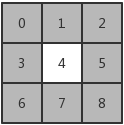
\includegraphics[width=0.2\textwidth]{images/cuda_fl/1}
	\caption{original access pattern(r=1)}
	\label{fig:cuda_fl_1}
\end{figure}

而且这仅仅是一次循环所需要访问的像素量, 为了让更多的像素间产生相互联系, 我们往往需要进行多次循环, 通常采用的循环量为iter=20.

为了减少运算量,我们对该算法稍微进行改动,变为每个像素点仅搜索左侧和上侧固定半径内的像素点,同时增加一个"标签冒泡"(label propagation)的步骤, 让每个像素点顺着flooding产生的label链条向根部查找,直到查找到的像素的$\Delta LUV > color\_range$. 这样既方便并行,又有利于获得更好的空间局部性。

以上描述的算法中, 每个线程块访问的像素点如图\ref{fig:cuda_fl_2}所示. 阴影区域为需要读取的, 非本线程对应的像素.

\begin{figure}[H]    
	\centering
	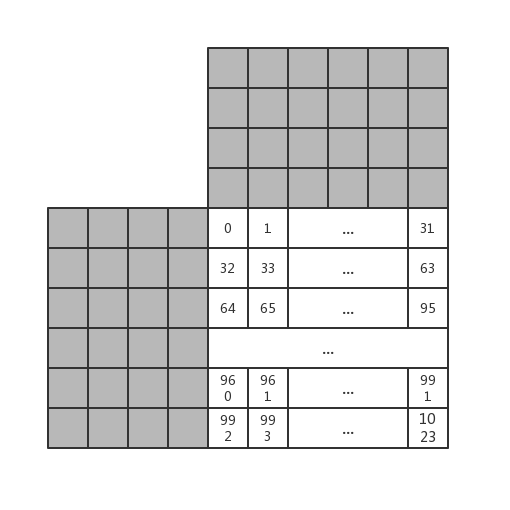
\includegraphics[width=0.4\textwidth]{images/cuda_fl/2}
	\caption{original access pattern(r=4)}
	\label{fig:cuda_fl_2}
\end{figure}

\subsubsection{加速结果}
\begin{enumerate}
	\item 我们首先实现了CPU单线程版本作为基准,
	使用640x480的灰度图像作为测试数据,经过profile,
	可得到CPU单线程版本的洪泛搜索耗时165ms。
	
	\item 然后我们将CPU单线程版本改为使用全局内存的CUDA版本,
	令每个CUDA线程处理一个像素点,经过profile,可得到使用全局内存的CUDA版本的洪泛搜索耗时490us,
	实现了约337倍的加速。
	
	\item 接下来我们利用GPU的共享内存来存放子图像素,经过改进后,
	得到利用共享内存的CUDA版本的洪泛搜索,经过profile,耗时202us,实现了约816倍的加速。
	
	\item 之后我们在翻阅代码的过程中发现,对比差异仅需进行一次,之后可以仅对标签进行冒泡,
	于是我们将代码重构,让洪泛搜索中的搜索和冒泡分离出来,经过profile,耗时215us,
	反而比没优化之前耗时更多。我们对这个现象感到好奇,经过一番对比和分析
	,最终找到了原因:我们每次冒泡都调用一次冒泡核函数,但由于显卡的机制,
	当显卡执行完当前核函数后,当前核函数所使用的缓存会被无效化,
	导致每次执行冒泡核函数都需要进行全局内存访问,因此拖累了运行时间。
	对此,我们将循环置于核函数内部,经过profile,耗时119us,最终实现了约1387倍的加速。
\end{enumerate}

产生的效果如图\ref{fig:cuda_fl_3}所示:

\begin{figure}[H]
	\centering
	\begin{subfigure}[b]{0.3\textwidth}
		\centering
		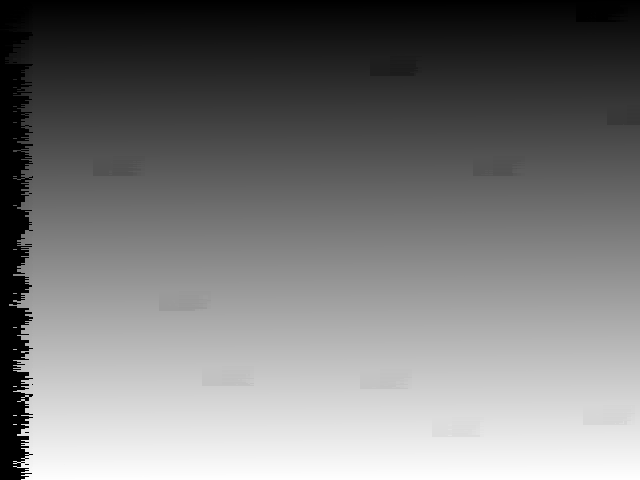
\includegraphics[width=\textwidth]{images/cuda_fl/result/3.png}
		\caption{iter=3}
	\end{subfigure}
	\hspace{5mm}
	\begin{subfigure}[b]{0.3\textwidth}
		\centering
		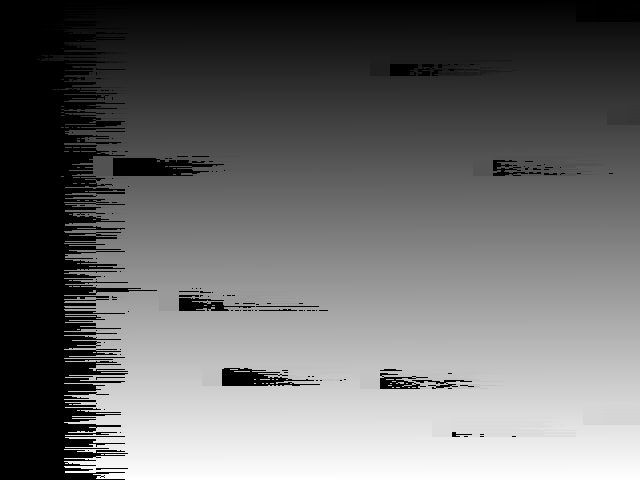
\includegraphics[width=\textwidth]{images/cuda_fl/result/5.png}
		\caption{iter=5}
	\end{subfigure}
	
	\begin{subfigure}[b]{0.3\textwidth}
		\centering
		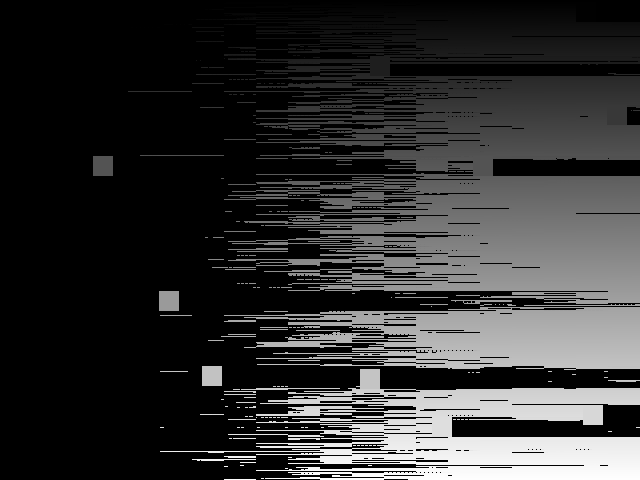
\includegraphics[width=\textwidth]{images/cuda_fl/result/7.png}
		\caption{iter=7}
	\end{subfigure}
	\hspace{5mm}
	\begin{subfigure}[b]{0.3\textwidth}
		\centering
		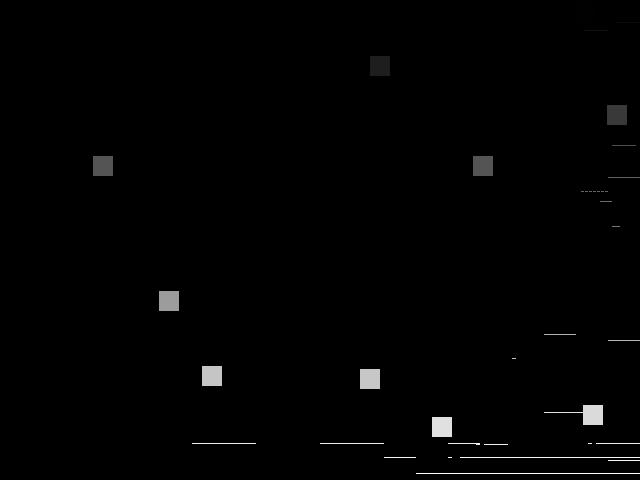
\includegraphics[width=\textwidth]{images/cuda_fl/result/9.png}
		\caption{iter=9}
	\end{subfigure}
	
	\caption{flooding result}
	\label{fig:cuda_fl_3}
\end{figure}


\subsection{区域合并的并行化}
\subsubsection{CUDA加速}
本节中,我们将对我们方法的CUDA核函数进行描述,我们的算法基于\autocite{DBLP:journals/corr/abs-1708-08180}中描述的UnionFind算法进行改进。我们使用了三个核函数,每个核函数的功能如下:
\begin{enumerate}
    \item 第一个核函数基于局部UF合并,通过使用共享内存来提升数据的访问速度,局部合并为最后的全局合并降低了复杂度
    \item 第二个核函数对每块的边界进行分析和合并,建立块与块之间的连接关系
    \item 第三个核函数对所有块进行全局合并,得到最终结果
\end{enumerate}

\textbf{A. 局部UF合并}

\begin{figure}[H]
	\centering
	\begin{subfigure}[b]{0.3\textwidth}
		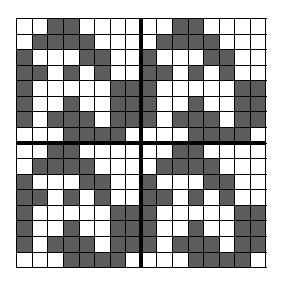
\includegraphics[width=\textwidth]{images/cuda_uf/uf_1.eps}
		\caption{input data}
		\label{fig:cuda_uf_1}
	\end{subfigure}
	\hspace{1mm} 
	\begin{subfigure}[b]{0.3\textwidth}
		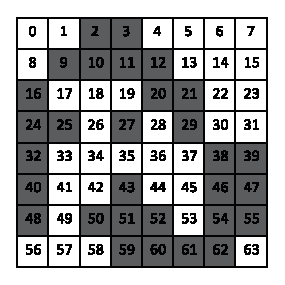
\includegraphics[width=\textwidth]{images/cuda_uf/uf_2.eps}
		\caption{initialized local label map}
		\label{fig:cuda_uf_2}
	\end{subfigure}
	\caption{Input data and initialized local label map}
\end{figure}

局部UF合并包括三个阶段:初始化,粗糙分类及行列归一化,局部UF。它的伪代码如\ref{code:cuda_uf_1}所示。

\begin{algorithm}[H]
	\setstretch{1.15}
	\DontPrintSemicolon
	\KwInput{经过Mean shift后的图片I}
	\KwInput{经过Flooding的labelIn}
	\KwInput{最大颜色区别colorRange}
	\KwOutput{最终经过聚合的labelOut}
	\KwDeclare{int\ $label_{sm}[],labelOrg_{sm},pixelBuff_{sm}$位于共享内存}
	\KwDeclare{int\ x,y,tid,gid,temp}
	x,y $\gets$ 2D\ global\ thread\ id \;
	\If{x>=imgWidth or y >= imgHeight}{
		\Return{}
	}

	\tcp{read data}
	tid $\gets$ 1D\ block\ thread\ id\;
	gid $\gets$ 1D\ global\ thread\ id\;
	$label_{sm}[tid]$ = tid\;
	$labelOrg_{sm}[tid]  = labelIn[gid]$
	$pixelBuff_{sm}[tid]$ = I[x,y]\;
	syncthreads()\;
	
	\tcp{row scan}
	\If{$||pixelBuff_{sm}[tid] - pixelBuff_{sm}[tid-1]||$ < colorRange} {
		$label_{sm}[tid] = label_{sm}[tid-1]$\;
	}
	syncthreads()\;

	\tcp{column scan}
	\If{$||pixelBuff_{sm}[tid] - pixelBuff_{sm}[tid-blockDim.x]||$ < colorRange} {
		$label_{sm}[tid] = label_{sm}[tid-blockDim.x]$\;
	}
	syncthreads()\;
	
	\tcp{row-column unification}
	temp $\gets$ tid\;
	\While{temp != $label_{sm}[temp]$}{
		temp $\gets label_{sm}[temp]$\;
		$\label_{sm}[temp]$ = temp\;	
	}
	
	\tcp{local union find}
	\If{$||pixelBuff_{sm}[tid] - pixelBuff_{sm}[tid-1]||$ < colorRange} {
		$unionFind(label_{sm}[], tid, tid-1)$\;
	}
	syncthreads()\;
	\If{$||pixelBuff_{sm}[tid] - pixelBuff_{sm}[tid-blockDim.x]||$ < colorRange} {
		$unionFind(label_{sm}[], tid, tid-blockDim.x)$\;
	}
	syncthreads()\;
	
	\tcp{store result}
	$label[gid] = labelOrg[label_{sm}[tid]]$\;
	\Return{图像I对应的label}
	\caption{区域合并算法}
	\label{code:cuda_uf_1}
\end{algorithm}

\clearpage
\textbf{1)初始化}

我们将图片分割成和线程块一样大小的若干块,如图\ref{fig:cuda_uf_1}所示,并且将每块分配给不同的线程块处理, 线程块通过共享内存来提升访问速度\autocite{cuda-toolkit-doc}, 函数读取原始的label到共享内存$labelOrg_{sm}$中方便最后查找, 并且初始化$label_{sm}$数组中元素为块内线程id, 一个初始化完毕的8x8大小的$label_{sm}$数组如\ref{fig:cuda_uf_1}所示.

\textbf{2)粗糙分类}

\begin{figure}[H]
	\centering
	\begin{subfigure}[b]{0.3\textwidth}
		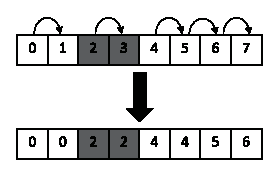
\includegraphics[width=\textwidth]{images/cuda_uf/uf_3.eps}
		\caption{row scan}
		\label{fig:cuda_uf_3}
	\end{subfigure}
	\hspace{5mm} 
	\begin{subfigure}[b]{0.3\textwidth}
		\hspace{9mm} 
		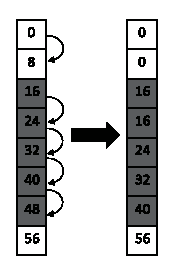
\includegraphics[height=\textwidth]{images/cuda_uf/uf_4.eps}
		\caption{column scan}
		\label{fig:cuda_uf_4}
	\end{subfigure}
	\caption{Scan model}
\end{figure}

在一个已经初始化的本地$label_{sm}$数组中, 左方和上方的像素点的label值总是小于当前像素点的label值的, 基于这个事实, 我们可以先进行行扫描, 融合同一行上相邻的像素点, 然后进行列扫描, 融合同一列上相邻的像素点, 图\ref{fig:cuda_uf_3}描述了行扫描的过程, 图\ref{fig:cuda_uf_4}描述了列扫描的过程. 这两种内存访问方式不会发生bank conflict,因此十分高效.

\textbf{3)行列归一化}
\begin{figure}[H]
	\centering
	\begin{subfigure}[b]{0.3\textwidth}
		\centering
		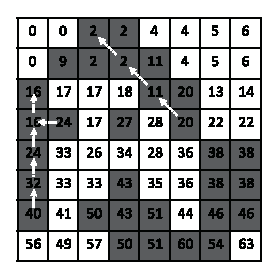
\includegraphics[width=\textwidth]{images/cuda_uf/uf_5.eps}
		\caption{local label map before row-column unification}
		\label{fig:cuda_uf_5}
	\end{subfigure}
	\hspace{5mm} 
	\begin{subfigure}[b]{0.3\textwidth}
		\centering
		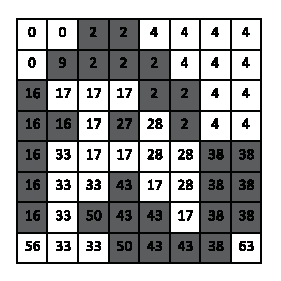
\includegraphics[width=\textwidth]{images/cuda_uf/uf_6.eps}
		\caption{local label map after row-column unification}
		\label{fig:cuda_uf_6}
	\end{subfigure}
	\caption{Coarse labeling}
\end{figure}

行列扫描后进行行列归一化, 归一化通过对块内每个像素调用$unionFind$算法完成像素点的标签统一, 此过程将根据行列扫描形成的邻接链条搜索最小局部label, 并更新像素点的值为此label. 因为线程块的大小受限于CUDA runtime, 因此这个查找过程的深度也是受限的, 另外, 使用共享内存也提高了访问效率.

\textbf{B. 边界分析}

\begin{figure}[H]
	\centering
	\begin{subfigure}[b]{0.6\textwidth}
		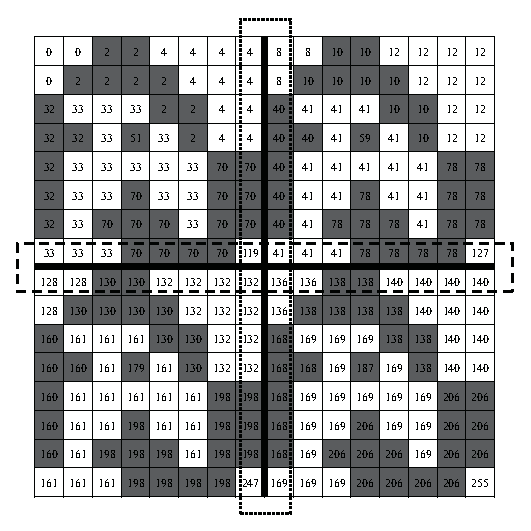
\includegraphics[width=\textwidth]{images/cuda_uf/uf_7.eps}
		\caption{global label map after local merge}
		\label{fig:cuda_uf_7}
	\end{subfigure}
	\hfill
	\begin{subfigure}[b]{0.6\textwidth}
		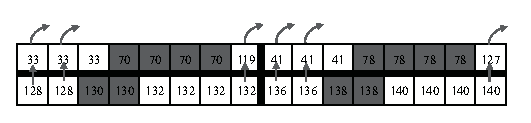
\includegraphics[width=\textwidth]{images/cuda_uf/uf_8.eps}
		\caption{boundary analysis along x-axis}
		\label{fig:cuda_uf_8}
	\end{subfigure}
	\caption{Coarse labeling}
\end{figure}

在边界分析阶段, 我们仅仅在每个块的邻接边上进行$unionFind$(图\ref{fig:cuda_uf_7}虚线框内), 为了节省线程数目和简化程序, 我们将边界分析拆分为水平(H)和竖直(V)两个阶段, 两个阶段的线程数目分别和水平与竖直方向各自邻接边的长素之和相等, 假设输入图片的分辨率为$N \times M$, 线程块大小为$\{b_x,b_y,1\}$, 则水平与竖直方向需要处理的像素数目(即线程数目)表示如下:

\begin{equation}
\begin{split}
P_x &= \floor{N/b_x} * M \\
P_y &= \floor{M/b_x} * N
\end{split}
\end{equation}

边界分析的伪代码如下:

\begin{algorithm}[H]
	\setstretch{1.15}
	\DontPrintSemicolon
	\KwInput{经过Mean shift后的图片I}
	\KwInput{经过Local merge的label}
	\KwInput{I的尺寸width,height}
	\KwInput{最大颜色区别colorRange}
	\KwDeclare{int\ x,y,gid}
	x,y $\gets$ 2D\ global\ thread\ id \;
	gid $\gets$ 1D\ global\ thread\ id \;
	\If{x>=imgWidth or y >= imgHeight}{
		\Return{}
	}
	
	\tcp{read data}
	
	\If{$||I[x,y] - I[x,y-1]||$ < colorRange} {
		unionFind(label[], gid, gid-width)\;
	}
	\Return{图像I对应的label}
	\caption{边界分析算法(H)}
	\label{code:cuda_uf_2}
\end{algorithm}

\begin{algorithm}[H]
	\setstretch{1.15}
	\DontPrintSemicolon
	\KwInput{经过Mean shift后的图片I}
	\KwInput{经过Local merge的label}
	\KwInput{I的尺寸width,height}
	\KwInput{最大颜色区别colorRange}
	\KwDeclare{int\ x,y,gid}
	x,y $\gets$ 2D\ global\ thread\ id \;
	gid $\gets$ 1D\ global\ thread\ id \;
	\If{x>=imgWidth or y >= imgHeight}{
		\Return{}
	}
	
	\tcp{read data}
	
	\If{$||I[x,y] - I[x-1,y]||$ < colorRange} {
		unionFind(label[], gid, gid-1)\;
	}
	\Return{图像I对应的label}
	\caption{边界分析算法(V)}
	\label{code:cuda_uf_2}
\end{algorithm}

\textbf{C. 全局合并}

在进行完边界分析后, 我们在全局内存上对所有像素点进行$unionFind$操作, 此时互相独立的局部标签被关联为一个这前提, 
我们使用和\autocite{Yonehara2015}以及\autocite{Oliveira2010}中一样的方法进行. 
此算法更具体的描述可以参考\autocite{Galler:1964:IEA:364099.364331}

\subsubsection{Pthread 加速}

本节中我们使用c语言的$<pthread.h>$库来实现union\_find多线程并行。
并行的思路跟cuda实现的union\_find类似。

\begin{algorithm}[H]
	\setstretch{1.15}
	\DontPrintSemicolon
	\KwInput{height,width}
	\KwInput{mode meanshift后的图像像素,一维float数组  }
	\KwInput{labels,color range,thread\_num}
	\KwOutput{new\_labels}
	
	block\_size=height*width/thread\_num \; 
    pthread\_data[thread\_num]  \;
    
    \tcp{img\_divide and partial\_union\_find }  \;
    \For{ i in range(0,thread\_num)} {
        start=i*block\_size  \;
        end=min(height*width-1,i*(block\_size+1)-1)   \;
        pthread\_data[i]=createPthreadData(start,end) \; 
    
        pthread\_create(pthread[1],partial\_union\_find\_function,pthread\_data[i])  \;

    }

    \tcp{wait for all thread end }
    \For{ i in range(0,thread\_num)}{ 
        pthread\_join(pthread[i])  \;
    }

    \tcp{boundary analysis  }
    \For{ i in range(0,thread\_num-1)}{  
        end=min(height*width-1,i*(block\_size+1)-1)  \;
        \For{ j in range(0,width)}{  \;
        \If{ color\_distance(mode[end-j],mode[end-j+width])<color\_range}{
            union\_find(end-j,end-j+width)  \;
        }}
    }
    \tcp{global\_merge } 


	\caption{Pthread区域合并算法}
\end{algorithm}

\textbf{A. 实现思路}

\begin{enumerate}
    \item 对于一个大小为height*width的图片,把图片分成height*width/THREAD\_NUM大小的THREAD\_NUM块,
    在每个子线程进行图片的局部并查集扩展
    \item 主线程处理边界问题,把边界上color\_distance相近的像素点所在的并查集合并起来
    \item 主线程通过归并排序把所有子线程的局部并查集进行最终合并,并对图像做重新标注,更新label
\end{enumerate}

在完成区域合并的实现之后, 我们还进行了性能评估, 
将我们所实现的并行版本的性能同串行版本的性能做了比较. 我们选取了若干张典型图片\ref{fig:uf_input}进行测试.


\begin{figure}[H]
    \centering
    \begin{subfigure}[b]{0.3\textwidth}
        \centering
        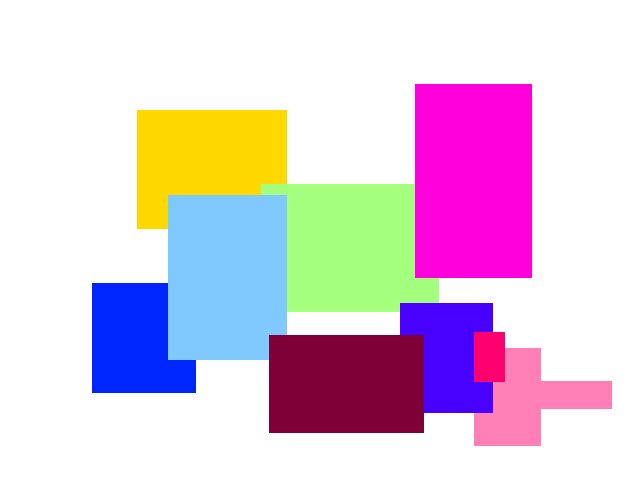
\includegraphics[width=\textwidth]{images/origin/1.png}
        \caption{test image 1, region=11}
    \end{subfigure}
    \hspace{5mm}
    \begin{subfigure}[b]{0.3\textwidth}
        \centering
        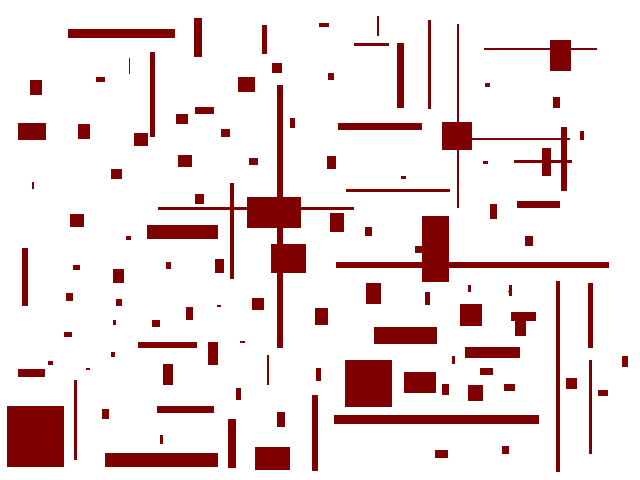
\includegraphics[width=\textwidth]{images/origin/2.png}
        \caption{test image 2, region=107}
    \end{subfigure}
    
    \begin{subfigure}[b]{0.3\textwidth}
        \centering
        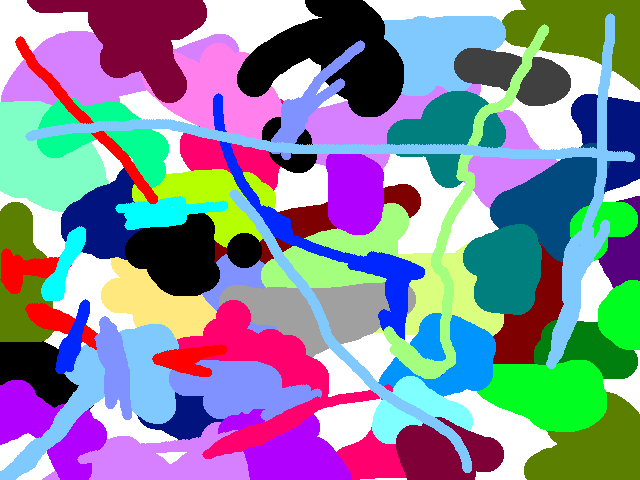
\includegraphics[width=\textwidth]{images/origin/3.png}
        \caption{test image 3, region=181}
    \end{subfigure}
    \hspace{5mm}
    \begin{subfigure}[b]{0.3\textwidth}
        \centering
        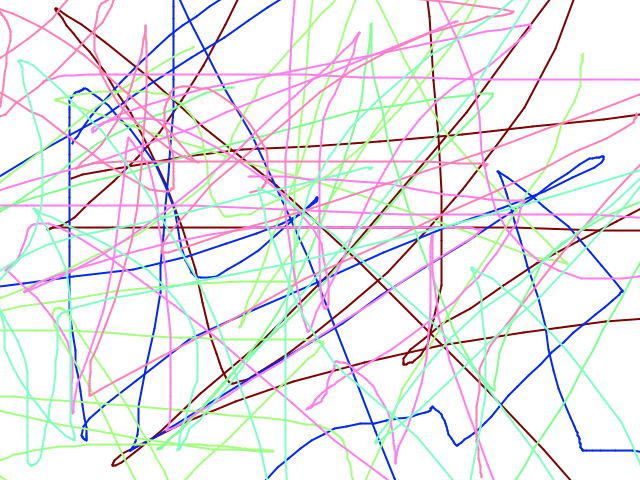
\includegraphics[width=\textwidth]{images/origin/4.png}
        \caption{test image 4, region=75592}
    \end{subfigure}
    
\caption{输入图片}
\label{fig:uf_input}
\end{figure}

\begin{figure}[H]
    \centering
    \begin{subfigure}[b]{0.3\textwidth}
        \centering
        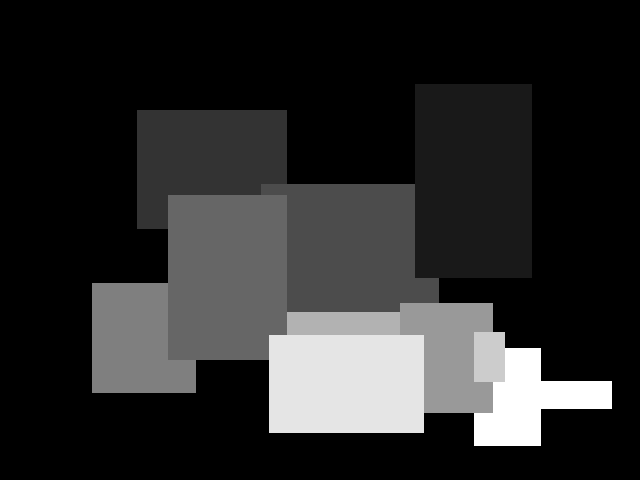
\includegraphics[width=\textwidth]{images/result/1.png}
        \caption{result of test 1}
    \end{subfigure}
    \hspace{5mm}
    \begin{subfigure}[b]{0.3\textwidth}
        \centering
        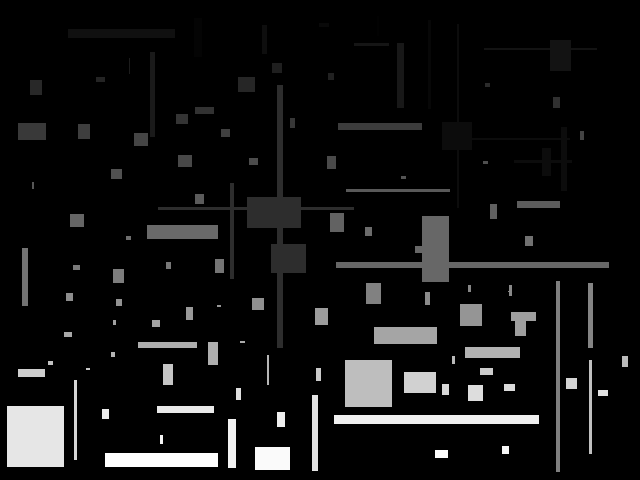
\includegraphics[width=\textwidth]{images/result/2.png}
        \caption{result of test 2}
    \end{subfigure}
    
    \begin{subfigure}[b]{0.3\textwidth}
        \centering
        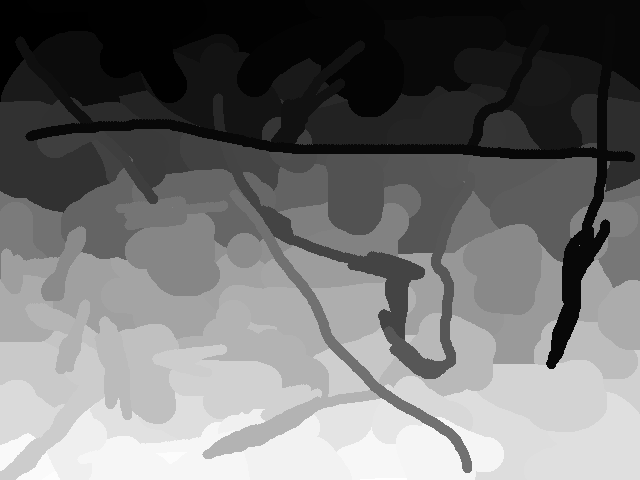
\includegraphics[width=\textwidth]{images/result/3.png}
        \caption{result of test 3}
    \end{subfigure}
    \hspace{5mm}
    \begin{subfigure}[b]{0.3\textwidth}
        \centering
        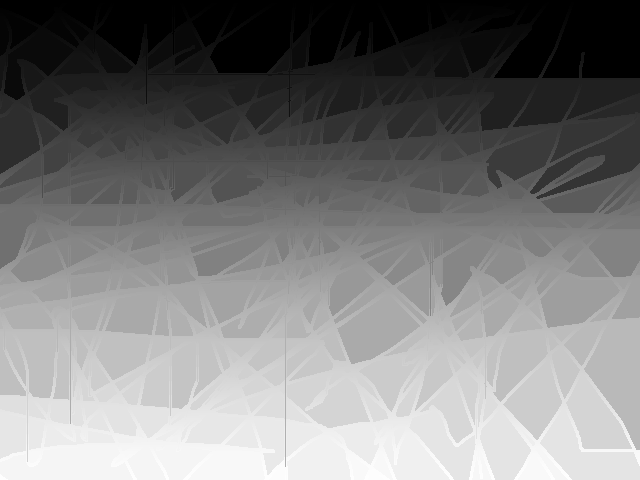
\includegraphics[width=\textwidth]{images/result/4.png}
         \caption{result of test 4}
    \end{subfigure}
\caption{输出图片}
\label{fig:uf_result}
\end{figure}

我们首先验证了两种算法的正确性, 输入图片经由区域合并算法的处理后, 
都得到了如图\ref{fig:uf_result}的输出. 经过程序核验, 可以确保所实现算法的正确性.


\textbf{A. Pthread加速效果}

在CPU为XEON E5 E5-2620 v4的平台上, 对四张图片分别进行五次单线程跟多线程的union\_find并统计运行时间,结果如表\ref{tb:pthread}
\begin{table}[H]
	\centering
    \begin{tabular}{cccccccc}
    \hline
    测试图像   & 线程数目 & 测试1(s) & 测试2(s) & 测试3(s) & 测试4(s) & 测试5(s) & 平均时间(s) \\ \hline
    1 & 1    & 0.153  & 0.144  & 0.149  & 0.149  & 0.148  & 0.1486    \\ \hline
    1 & 2    & 0.144  & 0.153  & 0.151  & 0.141  & 0.148  & 0.1474    \\ \hline
    1 & 4    & 0.152  & 0.139  & 0.142  & 0.137  & 0.143  & 0.1426    \\ \hline
    1 & 8    & 0.181  & 0.17   & 0.175  & 0.186  & 0.174  & 0.1772    \\ \hline
    2 & 1    & 0.145  & 0.143  & 0.153  & 0.145  & 0.143  & 0.1458    \\ \hline
    2 & 2    & 0.144  & 0.142  & 0.14   & 0.14   & 0.141  & 0.1414    \\ \hline
    2 & 4    & 0.176  & 0.134  & 0.14   & 0.137  & 0.138  & 0.145     \\ \hline
    2 & 8    & 0.176  & 0.172  & 0.178  & 0.172  & 0.166  & 0.1728    \\ \hline
    3 & 1    & 0.154  & 0.162  & 0.153  & 0.161  & 0.156  & 0.1572    \\ \hline
    3 & 2    & 0.156  & 0.144  & 0.157  & 0.151  & 0.146  & 0.1508    \\ \hline
    3 & 4    & 0.144  & 0.14   & 0.156  & 0.14   & 0.146  & 0.1452    \\ \hline
    3 & 8    & 0.184  & 0.18   & 0.184  & 0.189  & 0.184  & 0.1482    \\ \hline
    4 & 1    & 0.3    & 0.299  & 0.29   & 0.284  & 0.281  & 0.2908    \\ \hline
    4 & 2    & 0.279  & 0.265  & 0.269  & 0.27   & 0.281  & 0.2728    \\ \hline
    4 & 4    & 0.267  & 0.256  & 0.252  & 0.25   & 0.264  & 0.2578    \\ \hline
    4 & 8    & 0.313  & 0.316  & 0.316  & 0.327  & 0.328  & 0.32      \\ \hline
    \end{tabular}
    \caption{Pthread运行时间表}
    \label{tb:pthread}
\end{table}

    由表格我们知道多线程在线程数目为2或者4的时候性能最佳,
    但当线程数目继续增加时,由于线程创建销毁同步所需的时间更长,反而造成性能的下降。
接下来, 我们使用了一系列测试, 通过实验来测出我们所实现的并行算法的实际加速比. 
上述若干张图片的运行时间如下表所示.

\textbf{B. CUDA加速效果}

在GPU为TITAN X (Pascal)平台上, 块大小配置为\{32,32,1\}. CUDA版本的union find效果如表\ref{tb:union_find}所示
\begin{table}[H]
	\centering
	\begin{tabular}{cccc}
		\hline
		测试图像 & CPU单线程版本(ms) & GPU版本(ms) & 加速比 \\ \hline
		1       & 233.2           & 0.124       & 1881.4 \\ \hline
		2       & 232.4           & 0.127       & 1829.9\\ \hline
		3       & 243.1           & 0.126       & 1857.9 \\ \hline
		4       & 243.3           & 0.148      & 1643.9 \\ \hline
	\end{tabular}
	\caption{UnionFind运行时间表}
	\label{tb:union_find}
\end{table}


\clearpage
\section{Realtime test}
我们在CPU为i7 6700HQ, GPU为GTX 970m的平台上运行了连续的实时视频流处理测试, 所有CUDA核的块大小均配置为\{32,32,1\}, 在radius=16, color\_range=1000, connect\_color\_range=300的配置下, 单帧平均处理时间\textcolor{red}{28.32ms}, 运行结果如下

\begin{figure}[H]
	\centering
	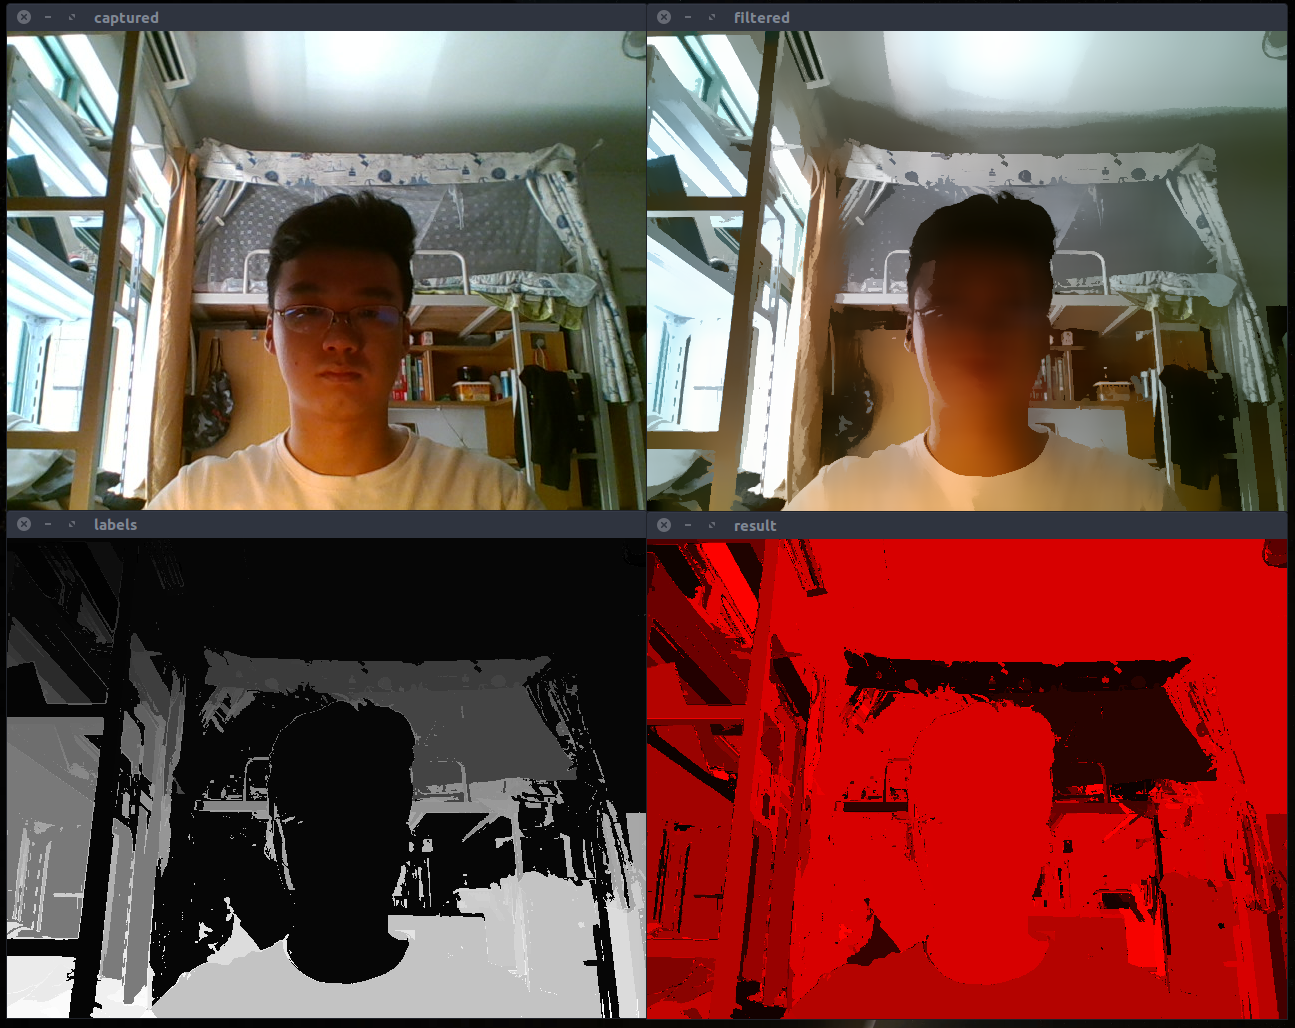
\includegraphics[width=1\linewidth]{images/realtime}
	\caption{realtime test}
	\label{fig:realtime}
\end{figure}

\clearpage

\section{Conclusion}
本次实验中我们实现了并行化的Mean Shift算法, 但是还是有一些不足之处, 

最后, 我们概括的总结一下我们小组在本次实验中的工作. 首先, 我们根据参考文献,
选取了Meanshift图像分割这一课题, 对它进行复现和并行化的优化. 在准备实验工作之前,
我们在开题报告时进行了充分的讨论和筹划, 并且在理论上重复了算法的推导过程,
验证了该算法的正确性和可靠性.

在实验中, 本小组成员分工明确, 配合紧密. 利用Github的pull-request-merge-branch等
机能进行了高效的团队协作, 在共同拟定出的接口文档, 测试规范, 算法模型等文件的指导下很好的实现了模块化
的分工和合作.

具体到实验设计上, 我们充分发挥了严谨认真的精神, 对于整个Meanshift算法的每个子模块, 都至少复现了串行版本和并行版本,
进行性能的对比实验. 有些部分还利用了CPU上的并行, 如某些模块还使用了OpenMP进行并行化等. 在每次实验中, 也充分发挥了
科学对照的精神, 每个模块都要求进行测试, 验证正确性. 同时在每个模块的效率考察上, 也务必做到多次重复实验取平均值,
控制并调整参数以取得最优表现等.

更重要的是, 在实验内容上, 我们成功并正确的复现了Meanshift滤波, Flooding, Union Find等一系列算法模块, 
所有模块都通过了正确性测试. 许多模块的CUDA加速版本比起串行版本, 都取得了相当巨大的加速成绩, 这里的具体内容可以
参照我们前文的实验报告. 而在CUDA加速的实现上, 我们软硬结合, 从算法考虑到GPU的内存, 架构采用了一系列优化措施.
比如有, 在Meanshift滤波中采用纹理内存, 共享内存; 在许多循环中使用了循环展开; 考量程序的时空局部性等等.


总的来说, 在本小组各成员的紧密配合, 有效协作下, 本次实验取得了比较完满的成功. 但也要看到, 我们的项目仍然
有一些不足之处, 仍然有可以优化的空间. 比如不能自适应, 需要一些超参数, 不能很好适应不同大小和纹理的图片, 
敏感度高分割会分出很多噪点, 敏感度低又会损失细节等. 在日后的学习工作中, 如果有机会, 我们将进一步完善我们的
工作, 力求做得更好.




\clearpage
\medskip
\printbibliography

\clearpage
\appendix
\section{个人报告}
\subsection{16337180麦显忠}
本次项目中我负责了unio\_find模块的多线程并行模块,这一模块用c的pthread库来实现多线程,目的是为了跟CUDA版本的union\_find做性能比较。基本的并行化思路是对图片进行分割,在子线程对图像的局部做label的合并,最后在主线程进行边界分析跟区域合并。

在这次项目中自己首次接触了用Cmake来组织项目,Cmake虽然比较繁琐,但对项目模块化十分有利,每个人只需要编译自己的Cmake文件就可以运行自己的模块,不会对队友的模块产生任何影响。

最后一点,感谢沐晗同学对我们的指导,虽然我是名义上的队长,但实际很多工作是沐晗在组织推进的。我自己也通过这次项目体会到一套完整的项目开发流程,像代码的组织、模块的划分、编程规范的规定、接口的规定、提交代码后他人的review,希望以后在团队项目中能用上这次项目的开发经验,与他人有跟愉快的合作开发。
\subsection{16313018李沐晗}
本次实验中,我所做的工作如下:
\begin{enumerate}
    \item 创建并维护项目的接口文档,编码规范等文档
    \item 创建并维护项目的cmake文件,维护项目的文件结构
    \item 为项目的每个模块查找合适的并行算法
    \item 设计项目的各个模块及测试程序和测试脚本,设计各个算法并行方法
    \item 编写项目的CUDA union find算法模块
    \item review其它同学的代码,提供详细的设计和优化建议
\end{enumerate}
本次项目比较棘手的地方是,每个模块有多种算法可供选择,而算法与算法之间的效率差异非常显著,同时针对每一种算法,又需要不同的并行方法,因此设计的工作是比较复杂的。比如我负责的模块功能是区域连接(第三阶段),我初始想法是把这个问题处理成一个min-cut问题,并了解了push-relabel算法,但发现这种算法不适合修改来适应不确定的多个区域的分割和区域内融合的需求,所以放弃,后来了解到了适合CUDA并行的union find算法,发现非常适合我的模块需求,因此采用了这个算法来进行并行。对于第二阶段的flooding算法,我也考虑了一些时间,最后选择设计成 “向左看,向上看” + “标签冒泡” 这样的方法来提高循环的效率。

第二个比较麻烦的地方是,指导其它同学时,传达自己的想法比较困难,尤其是对于CUDA这种非常依赖于访问模式的并行化方法,经常需要花费大量时间来详细描述每个线程的访问模式,因此在review的过程中,我发现缺乏一种有效的工具来告诉他人如何来写。

最后一个地方就是多人合作C++项目需要非常严格的接口规范和项目代码维护及检查,这一点上,我觉得我们做的还不够好,我虽然给出了初始的设计模板及代码规范,但后来发现在迭代过程中做了很多的修改,导致前面的设计完全不适用了,而且代码风格统一也需要比较多的精力,不过我通过加大review的力度及与其它同学的沟通交流解决了这个问题。

综上所述,在本次项目中我还是学习到了比较多的CUDA程序设计及合作经验的,希望以后的工作中能够用上本次项目的实践经验,做得更加完善。
\subsection{16337242韦博耀}
在本次项目中我负责了洪泛搜索模块的实现和优化。
我对原始的flooding算法进行了部分改进,使之更加适合CUDA并行化。之后按顺序逐步实现了CPU和GPU版本,并对GPU版本进行了优化。在优化过程中,我了解到了许多有用的调试、profile等工具,例如利用了cuda-memcheck来检查内存错误,利用nvprof来进行profile,利用cuda-gdb来进行调试。除此之外,我在优化代码时对代码进行了重构,但结果却比优化前要差,这就促使我去寻找更加深层的原因,最终对GPU内部的结构有了更加深刻的认识,从而成功优化了代码,最终结果跟CPU版本相比实现了1387倍的加速。

除此之外,本次项目使我对怎样进行高效的CUDA变成有了更加深刻的认识,例如利用好IDE提供的功能,充分进行模块化组织,编写好单元测试与集成测试,同时还有怎样高效地查阅官方文档。在本次项目中,CUDA官方文档给予了我巨大的帮助,使得我能够更好地编写CUDA代码。

还有一点就是Cmake的使用。虽然在日常学习中已经习惯了CMake的使用,但本次项目中CMake的使用方法还是让我眼前一亮,这样的组织方式和使用方法还是好评,让我学习到了许多新的操作,大大提升了我对使用CMake的经验。

最后,感谢沐晗同学在本次项目中对我的帮助。通过学习沐晗同学的项目组织、代码和优化思路,我学习到了许多新的东西,同时也得知了优秀的编程规范和项目组织方式,还有各种高效的编程方法。

\subsection{16337259谢江钊}
在本次项目中我主要负责了Meanshift模块的实现和后续的并行优化,这一部分的难点在于尽管它的算法并不复杂,但是并行的优化上来说还是有充分的思考空间的。从最开始的简单的一个像素一个线程,到后来考虑纹理内存提高内存的存取速度,然后发现block内部读取的范围一致使用共享内存提高速度,最后针对循环内部进行展开,以及还有减少强制转换提高速度,都做了很多各种各样的努力。而最终的结果也是非常优秀的,而最开始的没有做任何处理的优化,时间足足是现在的三十倍。CUDA内部的优化方法是丰富的,比起之前的小作业,这个大项目更加充分地让我掌握到一些优秀的优化技巧,同时也非常感谢沐晗同学的付出与指导,在这个项目中帮助了许多。

另外一点是这个项目采用了Camke来组织项目的配置,各个模块之间的调用,实现,声明都被区分开来,这种做法其实对我来说还是第一次接触,还有一些C调用CUDA的手段,利用模板去避免潜在的编译问题对我来说也是挺新颖的,因此在这些方面踩了不少的坑也学会了不少相关的知识。

最后一点是这次项目合作的地方我也觉得还有可以改进的地方,对接口的规范,文档组织和代码风格都可以进一步形成系统的解决方案。综上,我还是从这次项目中学习应用到了非常丰富的CUDA优化知识和团队合作经验,希望在以后的项目中能够吸收这次的经验。

\subsection{16337179麦金杰}
在本次项目中, 我主要负责开题报告以及结题报告的撰写, 整合, 加工等工作, 同时还参与了性能评测部分的工作. 总的来说, 因为我的分工中没有涉及到较多的实验和代码编写部分,
因此相对来说我的任务在小组中是比较轻松的. 因此在这里, 首先要感谢其它负责实验的同学的付出, 没有他们的付出和劳动, 是不可能写出这样一份详尽而充实的实验报告的.

在编写开题报告的过程中, 当时的主要参考paper是\cite{comaniciu2002mean}. 为了撰写报告和参与之后的工作的需要仔细阅读了这篇paper, 对于我们在本次实验所复现的Meanshift算法在理论层面有了比较深的认识和体会. 总的来看, 原文的重心其实在于推导和论证, 而并非算法的具体步骤或者实现. 这其实就给了我们的后续实现比较大的优化空间.  作者采用核密度估计的方法步步推导, 论证了朝Mean shift方向进行移动, 进行图像分割的理论基础和有效性. 我的认识和体会就是,作为深度学时代之前方法, 虽然它有着分割区块比较细碎, 受噪声和图像局部信息影响大等等缺点, 但它有着扎实的理论基础, 可以达到相当快的运算速度.

在我参与性能评测的过程中, 由于我们实现了独立而完整的测试模块, 这就使得我进行性能评测时, 调用各模块代码, 与串行模块对比, 检查输出和计时等变得相当方便. 体会到了在项目中引入测试模块, 基准评价体系的便捷和重要性.

在我完成结题报告的过程中, 采取了在Overleaf线上写作\LaTeX 文档的方式. 这不仅使得各成员间可以进行有效的沟通, 快速检查报告的内容和进度, 
同时基于LaTex的文档也让我们在算法的描述, 报告内容组织上更加得心应手. 而与此同时, 在整合各成员的实验工作, 与同伴进行算法和实验细节上的交流过程中, 也令得我对于整个算法既有比较宏观的整体把握, 也了解了更多项目实现过程中的具体细节, 比方说实验中遇到的困难, 各个模块间是如何优化的等等. 从总结他人的实验工作中也受益良多.

最后, 感谢所有人的付出 !!!


\end{document} 


%%% Local Variables:
%%% mode: latex
%%% TeX-master: t
%%% End:
